\section{Dataset Analysis and Experiments}
\subsection{Dataset Preparation and Preprocessing}
\begin{minted}{py}
def split_and_visualize(X, y, dataset_name: str):
    splits = {}

    for ratio in [0.4, 0.6, 0.8, 0.9]:
        X_train, X_test, y_train, y_test = train_test_split(
            X, y, train_size=ratio, stratify=y, shuffle=True, random_state=42
        )

        splits[ratio] = (X_train, X_test, y_train, y_test)

    return splits
\end{minted}
\begin{flushleft}
	To shuffle the dataset and ensure it is split in a stratified fashion, we use the \texttt{train\_test\_split} function from \texttt{sklearn.model\_selection}. The function takes the dataset and the target variable as inputs, along with the desired train-test split ratio.
	\begin{itemize}
		\item The \texttt{shuffle} parameter randomizes the order of the samples before splitting.
		\item The \texttt{stratify} parameter ensures the dataset is split in a stratified fashion.
	\end{itemize}
\end{flushleft}

\subsection{Interpreting Classification Report and Confusion Matrix}
\begin{minted}{py}
def train_evaluate_decision_tree(
    X_train,
    y_train,
    X_test,
    y_test,
    dataset_name: str,
    split_ratio,
):
    # Dynamically set feature and class names
    feature_names = X_train.columns.tolist()
    class_names = [str(cls) for cls in np.unique(y_train)]

    # Train model
    clf = DecisionTreeClassifier(criterion="entropy", random_state=42)
    clf.fit(X_train, y_train)

    # Predictions
    y_pred = clf.predict(X_test)

    # Classification Report (with validation)
    print(f"\nClassification Report ({dataset_name}, {display_ratio(split_ratio)}):")
    print(
        classification_report(
            y_test,
            y_pred,
            target_names=class_names,
            labels=np.unique(y_test),  # Ensure alignment with actual classes
        )
    )

    # Confusion Matrix
    sns.heatmap(
        confusion_matrix(y_test, y_pred),
        annot=True,
        fmt="d",
        xticklabels=class_names,
        yticklabels=class_names,
    )
\end{minted}
\begin{flushleft}
	To generate the classification report and confusion matrix:
	\begin{itemize}
		\item The \texttt{classification\_report} function provides a detailed report of the model's performance, including precision, recall, and F1-score for each class.
		\item The \texttt{confusion\_matrix} function generates a matrix that shows the number of correct and incorrect predictions for each class.
	\end{itemize}
\end{flushleft}

\begin{flushleft}
	\begin{itemize}
		\item The classification report summarizes, for each class \(c\):
		      \begin{itemize}
			      \item \textbf{Precision} (\(\mathrm{Prec}_c\)): measures the fraction of samples predicted as \(c\) that truly belong to \(c\).
			      \item \textbf{Recall} (\(\mathrm{Rec}_c\)): measures the fraction of true-\(c\) samples correctly identified.
			      \item \textbf{F1-score} (\(\mathrm{F1}_c\)): the harmonic mean of precision and recall
			      \item \textbf{Support}: the number of true samples of class \(c\).
		      \end{itemize}
		\item For example, with a binary problem (classes “positive”/“negative”), the confusion matrix is:
		      \begin{flushleft}
			      \[
				      \mathbf{CM} =
				      \begin{pmatrix}
					      \mathrm{TN} & \mathrm{FP} \\
					      \mathrm{FN} & \mathrm{TP}
				      \end{pmatrix},
			      \]
			      where
			      \begin{description}
				      \item[\(\mathrm{TN}\) (True Negative):] correctly predicted negatives.
				      \item[\(\mathrm{FP}\) (False Positive, Type I error):] negatives incorrectly predicted as positives.
				      \item[\(\mathrm{FN}\) (False Negative, Type II error):] positives incorrectly predicted as negatives.
				      \item[\(\mathrm{TP}\) (True Positive):] correctly predicted positives.
			      \end{description}
			      \noindent From these entries we derive:
			      \begin{align*}
				      \text{Accuracy}                  & = \frac{\mathrm{TP} + \mathrm{TN}}{\mathrm{TP} + \mathrm{TN} + \mathrm{FP} + \mathrm{FN}}, \\
				      \text{False Positive Rate (FPR)} & = \frac{\mathrm{FP}}{\mathrm{FP} + \mathrm{TN}},                                           \\
				      \text{False Negative Rate (FNR)} & = \frac{\mathrm{FN}}{\mathrm{FN} + \mathrm{TP}}
			      \end{align*}
			      \begin{align*}
				      \text{Specificity (True Negative Rate)} & = \frac{\mathrm{TN}}{\mathrm{TN} + \mathrm{FP}}, \\
				      \text{Precision}                        & = \frac{\mathrm{TP}}{\mathrm{TP} + \mathrm{FP}}, \\
				      \text{Recall (Sensitivity)}             & = \frac{\mathrm{TP}}{\mathrm{TP} + \mathrm{FN}}
			      \end{align*}
			      \noindent A well‐performing classifier exhibits high \(\mathrm{TP}\) and \(\mathrm{TN}\), and low \(\mathrm{FP}\) and \(\mathrm{FN}\).
			      \begin{itemize}
				      \item \emph{High FP} indicates many false alarms.
				      \item \emph{High FN} indicates many misses—critical in domains such as medical diagnosis.
				      \item \emph{High FP} indicates many false alarms (\(\leq 15\%\)).
			      \end{itemize}
		      \end{flushleft}
	\end{itemize}
\end{flushleft}

%================ Breast Cancer =================%
\clearpage
\subsection{Breast Cancer Wisconsin Dataset}
\subsubsection*{Dataset Description}
\begin{itemize}
	\item \textbf{Description:} The UCI Breast Cancer Wisconsin (Diagnostic) dataset is used for classifying tumors as malignant or benign based on features derived from its imaging data.
	\item \textbf{Dataset Info:} 569 samples, binary labels (malignant vs.\ benign), 30 numeric features.
	\item \textbf{Preprocessing:} shuffle \& stratified split at 40/60, 60/40, 80/20, 90/10.
\end{itemize}

\begin{figure}[H]
	\centering
	\begin{subfigure}{0.45\textwidth}
		\centering
		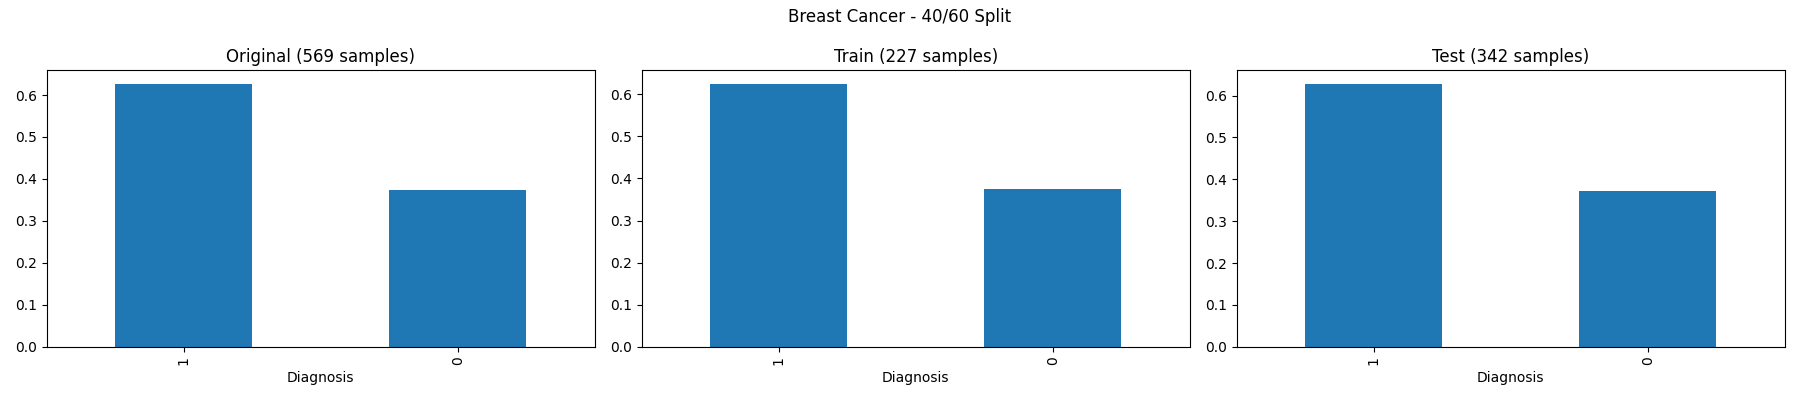
\includegraphics[width=\textwidth]{imgs/class_dist/class_dist__breast_cancer__40_vs_60.png}
		\caption{Breast Cancer: class distribution (40/60 split).}\label{fig:bc-cd-40-60}
	\end{subfigure}
	\hfill
	\begin{subfigure}{0.45\textwidth}
		\centering
		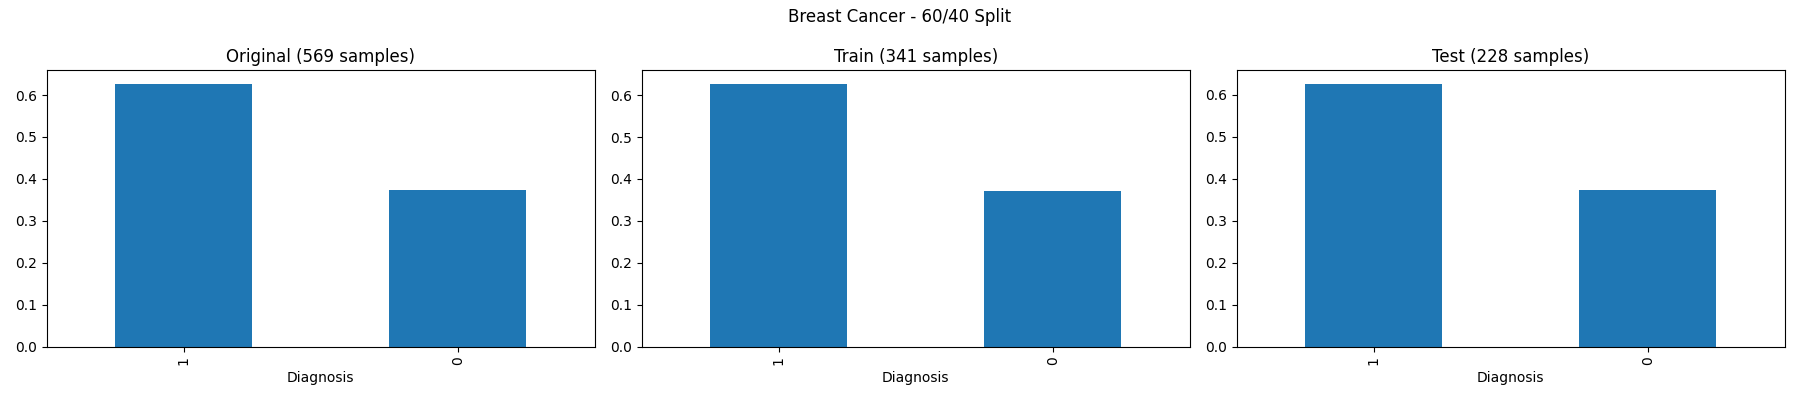
\includegraphics[width=\textwidth]{imgs/class_dist/class_dist__breast_cancer__60_vs_40.png}
		\caption{Breast Cancer: class distribution (60/40 split).}\label{fig:bc-cd-60-40}
	\end{subfigure}
	\hfill
	\begin{subfigure}{0.45\textwidth}
		\centering
		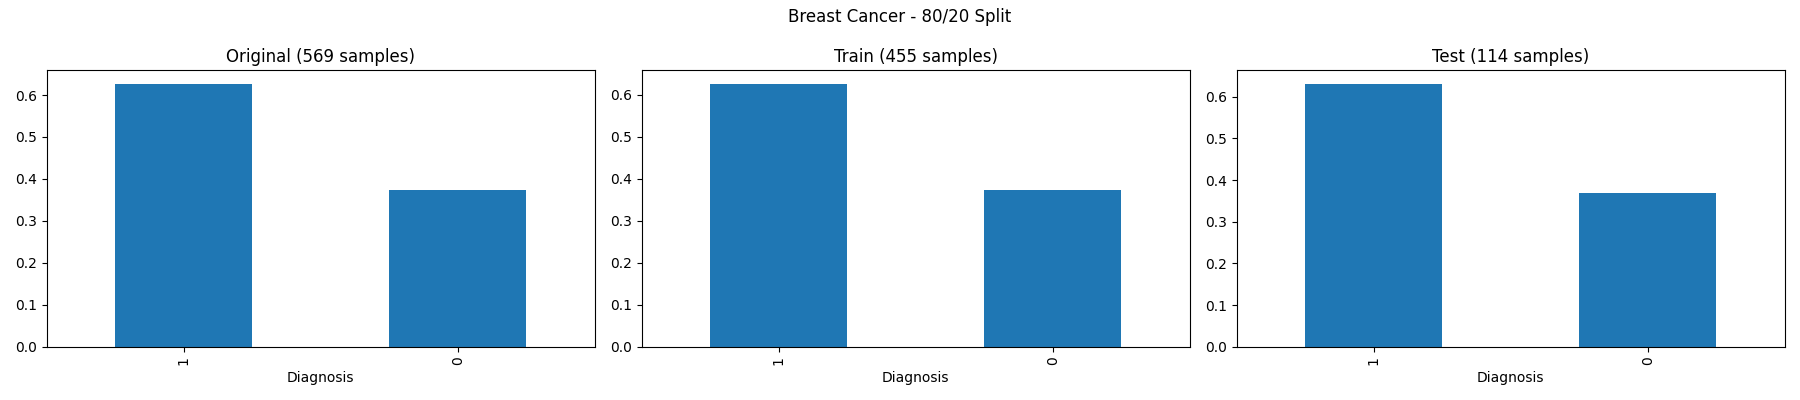
\includegraphics[width=\textwidth]{imgs/class_dist/class_dist__breast_cancer__80_vs_20.png}
		\caption{Breast Cancer: class distribution (80/20 split).}\label{fig:bc-cd-80-20}
	\end{subfigure}
	\hfill
	\begin{subfigure}{0.45\textwidth}
		\centering
		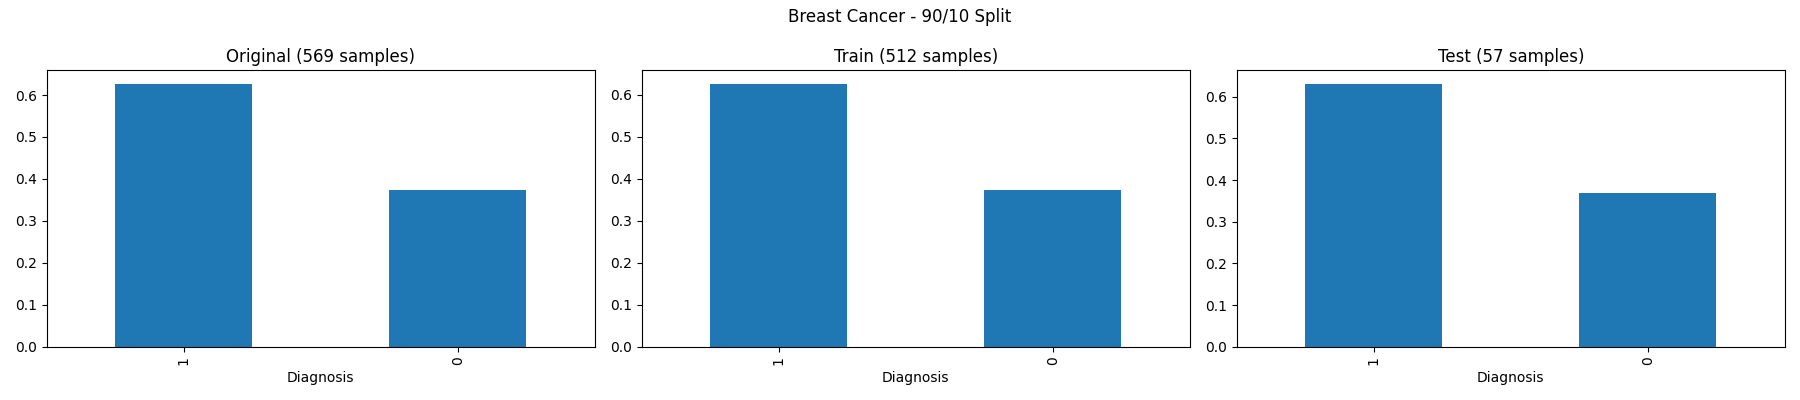
\includegraphics[width=\textwidth]{imgs/class_dist/class_dist__breast_cancer__90_vs_10.png}
		\caption{Breast Cancer: class distribution (90/10 split).}\label{fig:bc-cd-90-10}
	\end{subfigure}

	\caption{Class distributions}\label{fig:bc-cd-all}
\end{figure}

% \clearpage
% \subsubsection*{Building Decision Tree Classifiers for each train/test proportions}
% \begin{figure}[H]
% 	\centering
% 	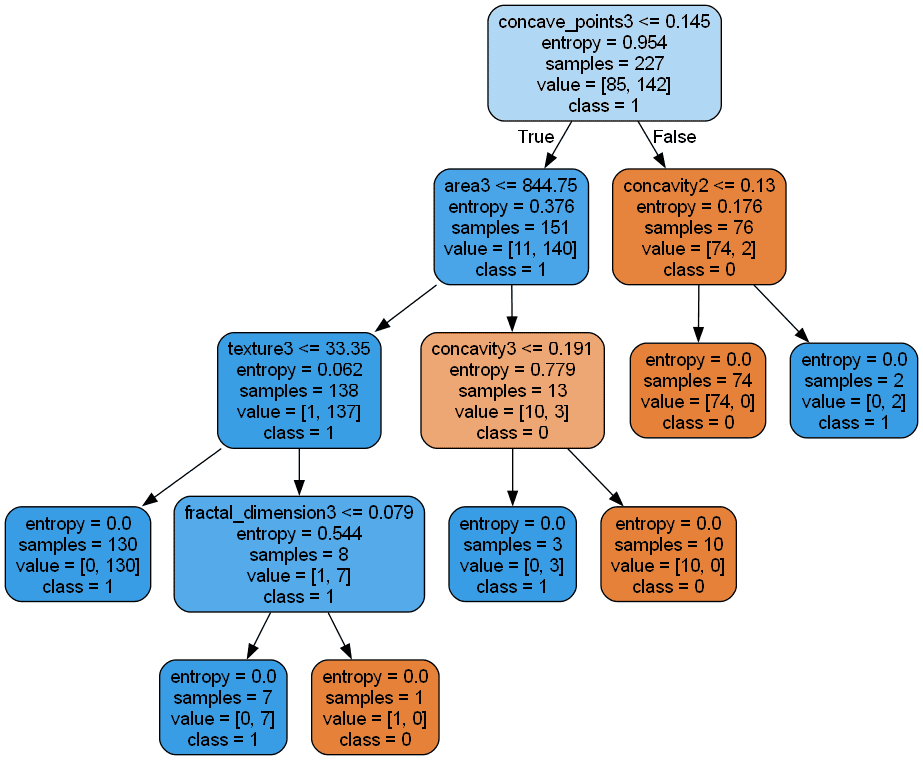
\includegraphics[width=0.65\textwidth]{imgs/dt-mini/dt__breast_cancer__40_vs_60.png}
% 	\caption{Breast Cancer: decision tree for 40/60 split.}\label{fig:bc-dt-40-60}
% \end{figure}
% \begin{figure}[H]
% 	\centering
% 	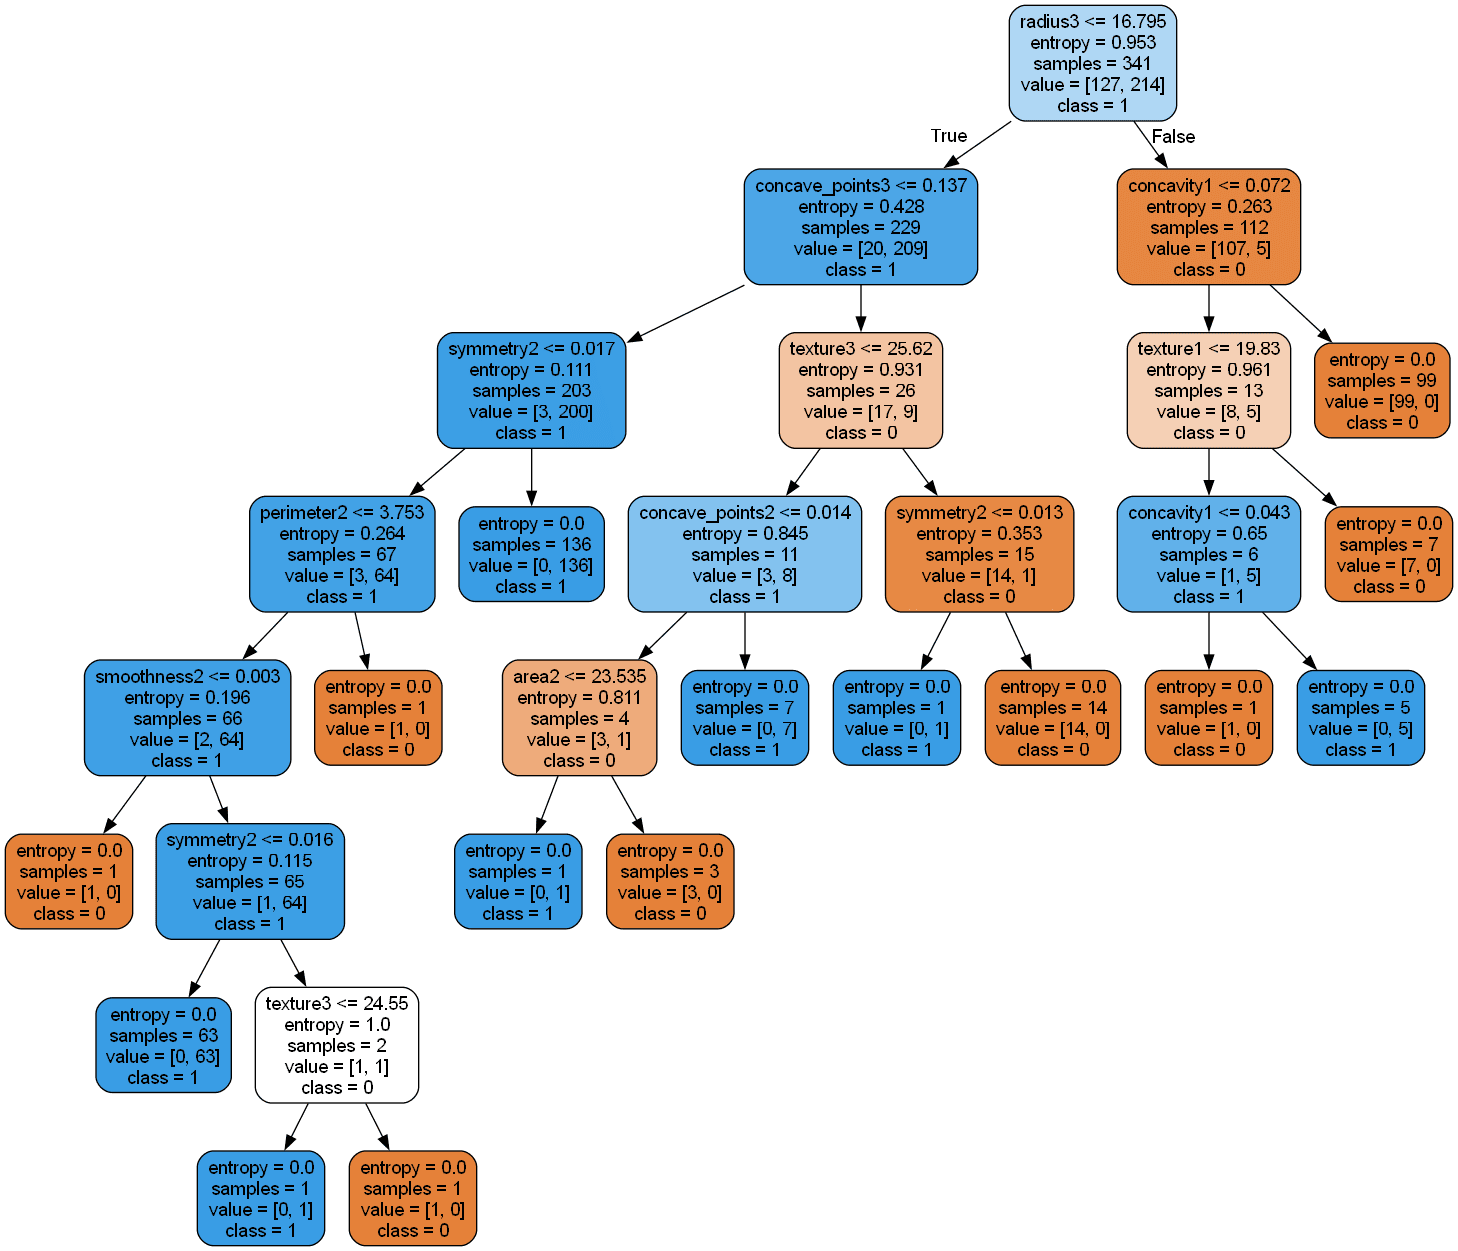
\includegraphics[width=0.65\textwidth]{imgs/dt-mini/dt__breast_cancer__60_vs_40.png}
% 	\caption{Breast Cancer: decision tree for 60/40 split.}\label{fig:bc-dt-60-40}
% \end{figure}
% \begin{figure}[H]
% 	\centering
% 	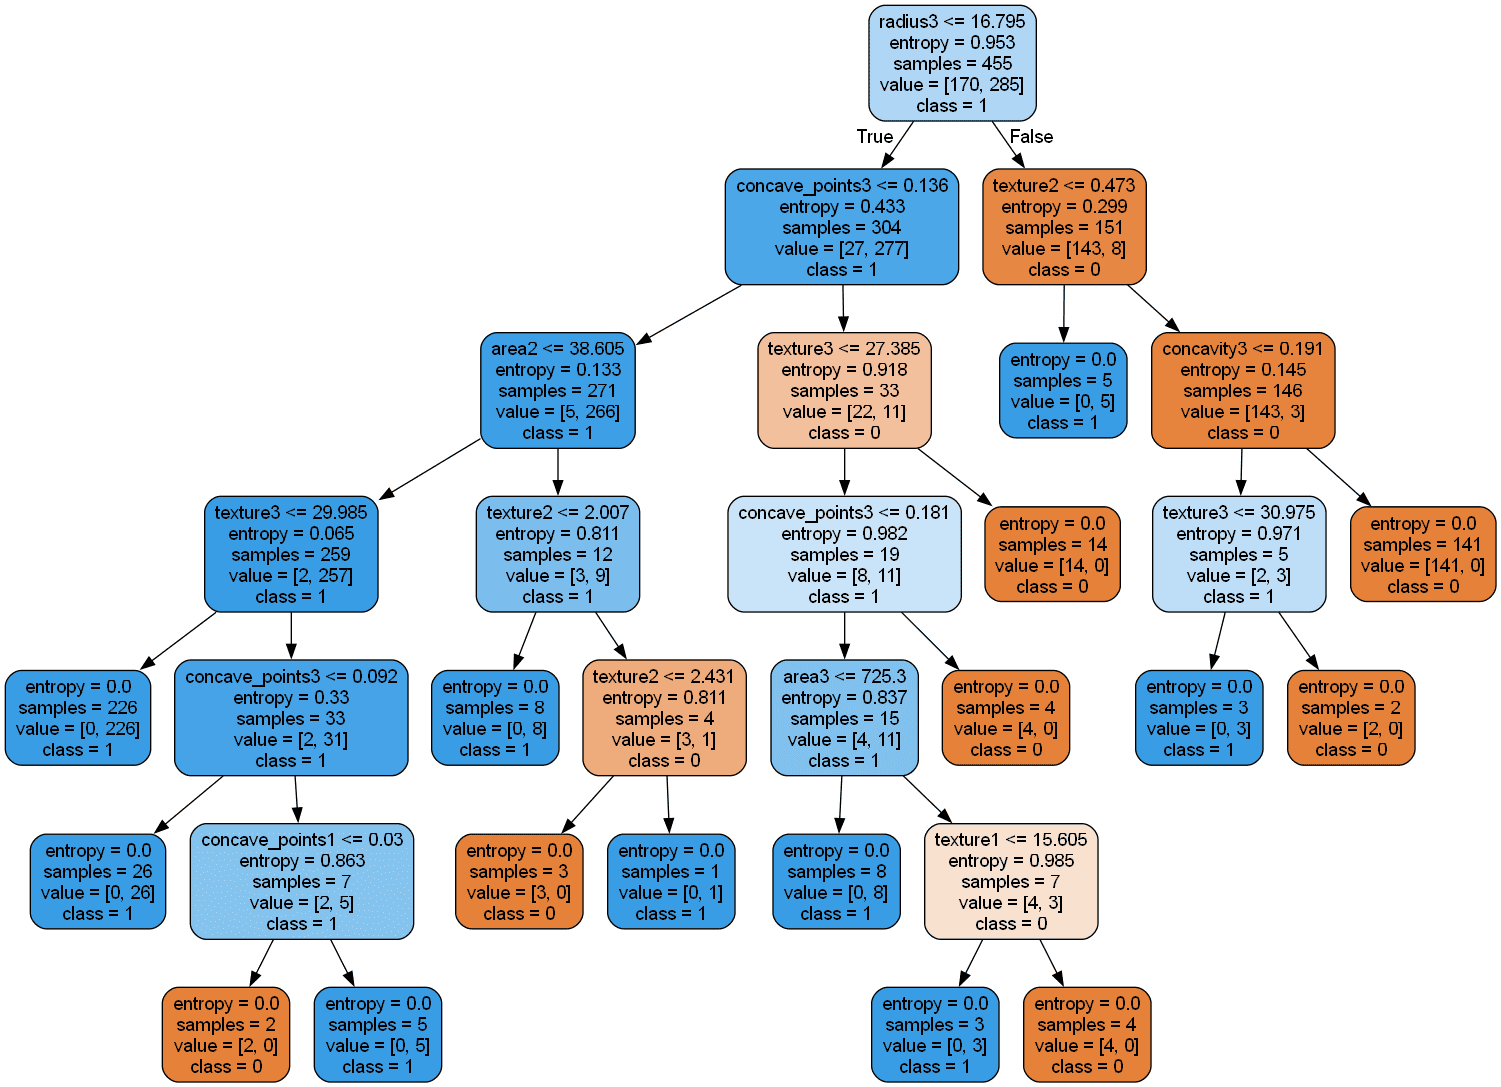
\includegraphics[width=0.65\textwidth]{imgs/dt-mini/dt__breast_cancer__80_vs_20.png}
% 	\caption{Breast Cancer: decision tree for 80/20 split.}\label{fig:bc-dt-80-20}
% \end{figure}
% \begin{figure}[H]
% 	\centering
% 	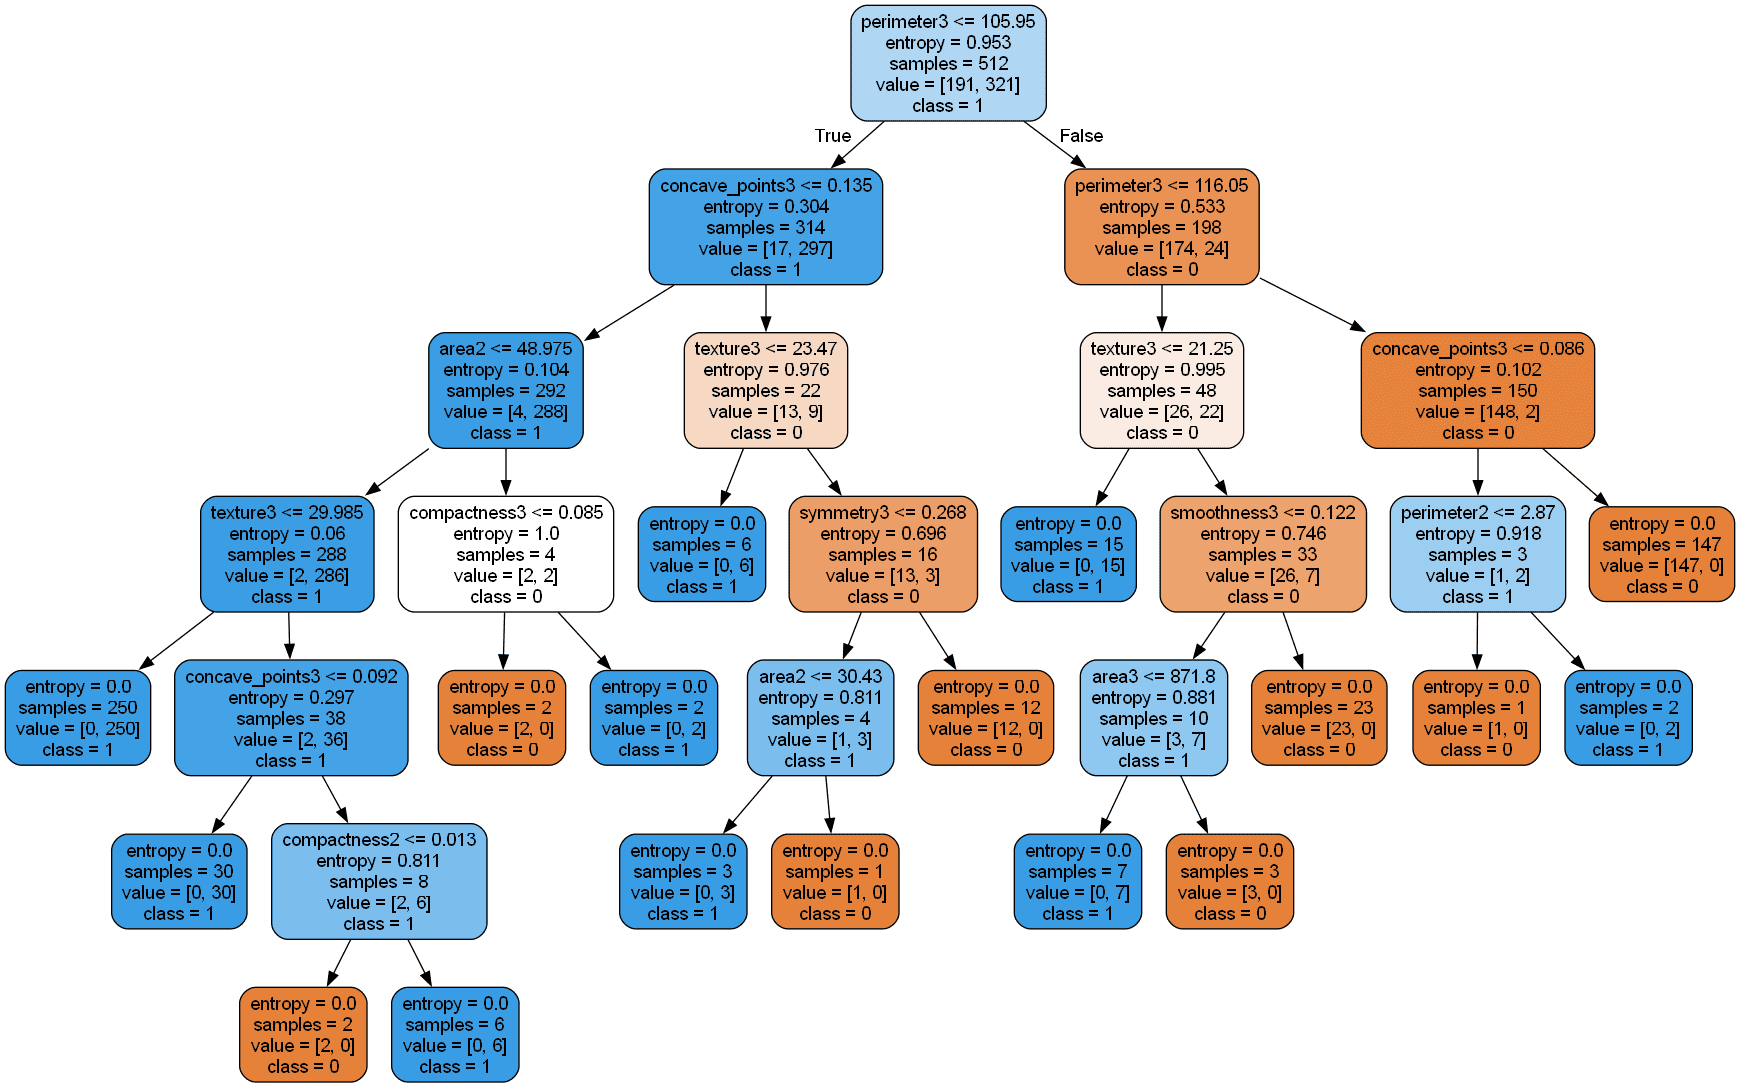
\includegraphics[width=0.65\textwidth]{imgs/dt-mini/dt__breast_cancer__90_vs_10.png}
% 	\caption{Breast Cancer: decision tree for 90/10 split.}\label{fig:bc-dt-90-10}
% \end{figure}

\clearpage
\subsubsection*{Evaluating the decision tree classifiers}
\begin{figure}[H]
	\centering
	\begin{subfigure}{0.45\textwidth}
		\centering
		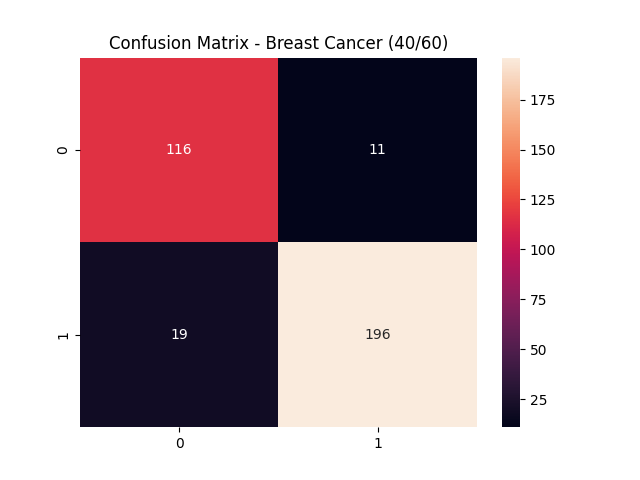
\includegraphics[width=\textwidth]{imgs/confusion_mat/confusion_mat__breast_cancer__40_vs_60.png}
		\caption{Breast Cancer: confusion matrix (40/60 split).}\label{fig:bc-cm-40-60}
	\end{subfigure}
	\hfill
	\begin{subfigure}{0.45\textwidth}
		\centering
		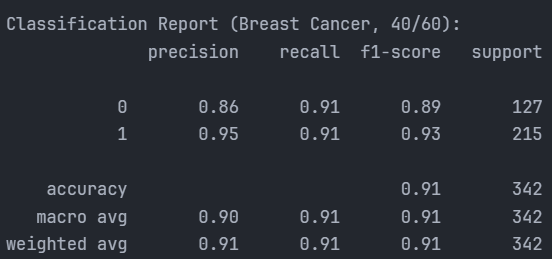
\includegraphics[width=\textwidth]{imgs/confusion_mat/class_rp__breast_cancer__40_vs_60.png}
		\caption{Breast Cancer: Classification Report (40/60 split).}\label{fig:bc-cr-40-60}
	\end{subfigure}

	\caption{Classification Report and Confusion Matrix (40/60 split)}\label{fig:bc-eval-40-60}
\end{figure}
\begin{figure}[H]
	\centering
	\begin{subfigure}{0.45\textwidth}
		\centering
		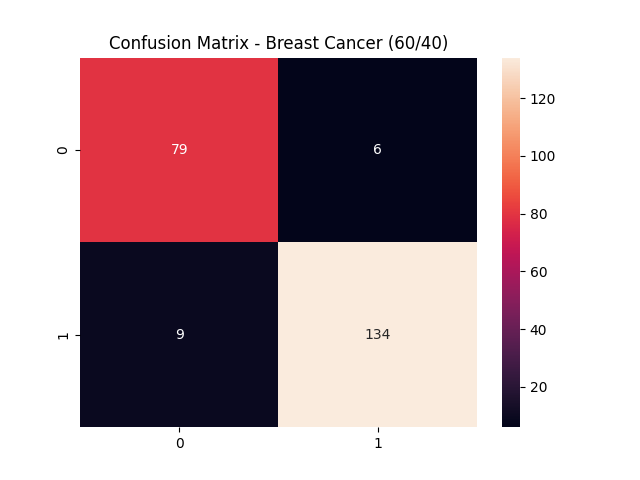
\includegraphics[width=\textwidth]{imgs/confusion_mat/confusion_mat__breast_cancer__60_vs_40.png}
		\caption{Breast Cancer: confusion matrix (60/40 split).}\label{fig:bc-cm-60-40}
	\end{subfigure}
	\hfill
	\begin{subfigure}{0.45\textwidth}
		\centering
		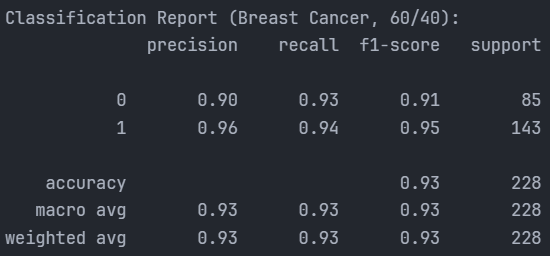
\includegraphics[width=\textwidth]{imgs/confusion_mat/class_rp__breast_cancer__60_vs_40.png}
		\caption{Breast Cancer: Classification Report (60/40 split).}\label{fig:bc-cr-60-40}
	\end{subfigure}

	\caption{Classification Report and Confusion Matrix (60/40 split)}\label{fig:bc-eval-60-40}
\end{figure}
\begin{figure}[H]
	\centering
	\begin{subfigure}{0.45\textwidth}
		\centering
		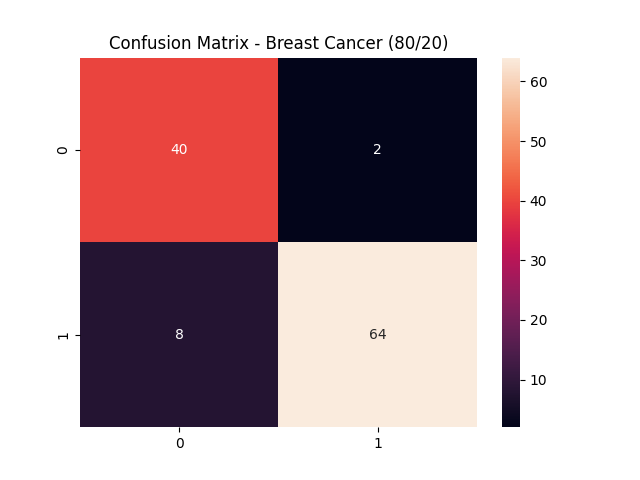
\includegraphics[width=\textwidth]{imgs/confusion_mat/confusion_mat__breast_cancer__80_vs_20.png}
		\caption{Breast Cancer: confusion matrix (80/20 split).}\label{fig:bc-cm-80-20}
	\end{subfigure}
	\hfill
	\begin{subfigure}{0.45\textwidth}
		\centering
		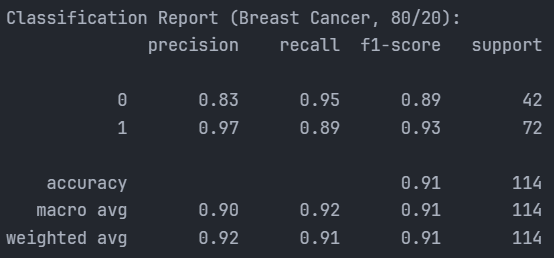
\includegraphics[width=\textwidth]{imgs/confusion_mat/class_rp__breast_cancer__80_vs_20.png}
		\caption{Breast Cancer: Classification Report (80/20 split).}\label{fig:bc-cr-80-20}
	\end{subfigure}

	\caption{Classification Report and Confusion Matrix (80/20 split)}\label{fig:bc-eval-80-20}
\end{figure}
\begin{figure}[H]
	\centering
	\begin{subfigure}{0.45\textwidth}
		\centering
		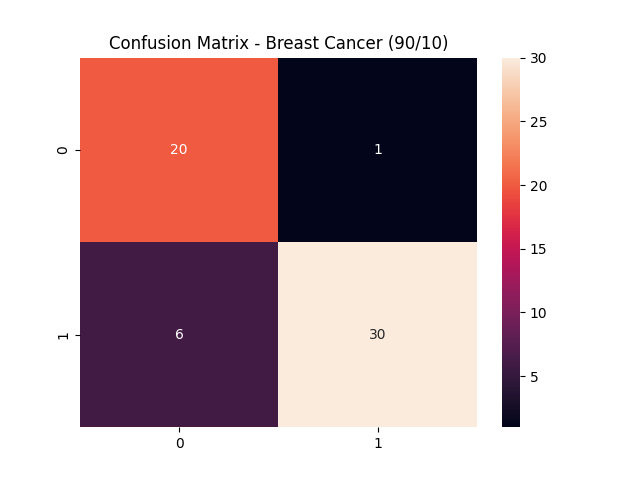
\includegraphics[width=\textwidth]{imgs/confusion_mat/confusion_mat__breast_cancer__90_vs_10.png}
		\caption{Breast Cancer: confusion matrix (90/10 split).}\label{fig:bc-cm-90-10}
	\end{subfigure}
	\hfill
	\begin{subfigure}{0.45\textwidth}
		\centering
		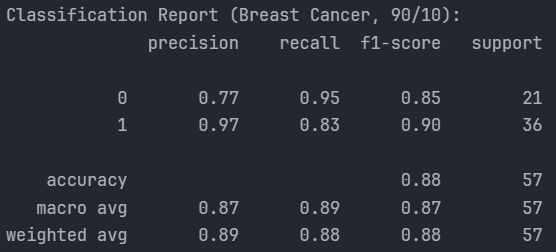
\includegraphics[width=\textwidth]{imgs/confusion_mat/class_rp__breast_cancer__90_vs_10.png}
		\caption{Breast Cancer: Classification Report (90/10 split).}\label{fig:bc-cr-90-10}
	\end{subfigure}

	\caption{Classification Report and Confusion Matrix (90/10 split)}\label{fig:bc-eval-90-10}
\end{figure}

\subsubsection*{Insights - Performance Evaluation}
\begin{itemize}
	\item \textbf{Accuracy by split ratio:}
	      \begin{itemize}
		      \item 60/40 split achieved the highest test accuracy at \textbf{93\%}.
		      \item 40/60 and 80/20 splits both reached \textbf{91\%}.
		      \item 90/10 dropped to \textbf{88\%}, showing increased variance with a very small test set.
	      \end{itemize}
	\item \textbf{Class-level performance:}
	      \begin{itemize}
		      \item \emph{Malignant (class 0):}
		            \begin{itemize}
			            \item Precision ranged from 0.86 (40/60) → 0.90 (60/40) → 0.83 (80/20) → 0.77 (90/10).
			            \item Recall stayed high (0.91, 0.93, 0.95, 0.95), ensuring most malignant tumors are detected.
		            \end{itemize}
		      \item \emph{Benign (class 1):}
		            \begin{itemize}
			            \item Precision consistently excellent (0.95-0.97), meaning very few benign cases are mislabeled malignant.
			            \item Recall varied from 0.91 (40/60), 0.94 (60/40), 0.89 (80/20) to 0.83 (90/10), indicating some benign samples get misclassified when test size shrinks.
		            \end{itemize}
	      \end{itemize}
	\item \textbf{Macro vs.\ weighted F1:} Both averaged around 0.91 for splits \(\geq\)40/60, dropping slightly for 90/10—indicating stable balanced performance except with very few test examples.
	\item \textbf{Clinical implication:}
	      \begin{itemize}
		      \item Keeping malignant recall \(\geq\)90\% is critical to minimize missed cancer diagnoses.
		      \item A benign precision \(\geq\)85\% keeps false alarms at a manageable level in screening programs.
	      \end{itemize}
\end{itemize}

\clearpage
\subsubsection*{Decision Tree Classifier with Different Depths}
\begin{figure}[H]
	\centering
	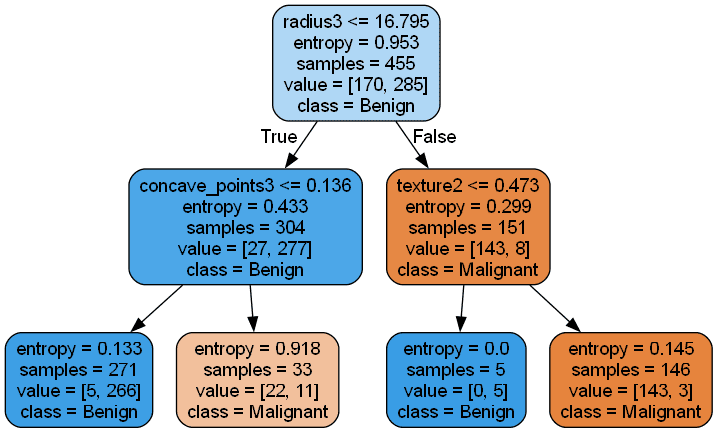
\includegraphics[width=0.65\textwidth]{imgs/dt-mini/dt__breast_cancer__80_vs_20__2.png}
	\caption{Breast Cancer: decision tree with \texttt{max\_depth}=2 (80/20 split).}\label{fig:bc-dt-depth-2}
\end{figure}

\begin{figure}[H]
	\centering
	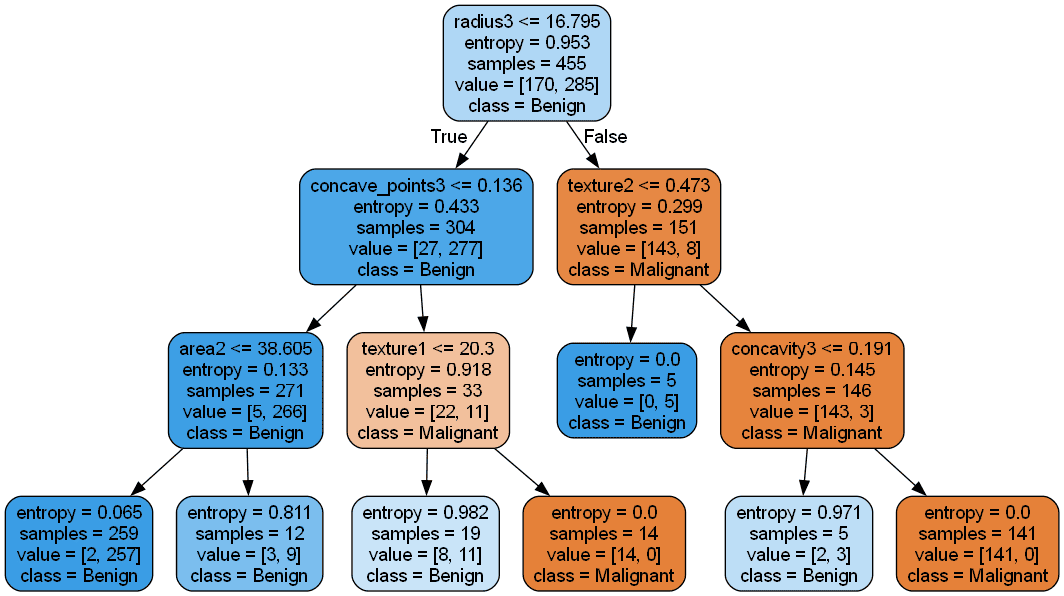
\includegraphics[width=0.65\textwidth]{imgs/dt-mini/dt__breast_cancer__80_vs_20__3.png}
	\caption{Breast Cancer: decision tree with \texttt{max\_depth}=3 (80/20 split).}\label{fig:bc-dt-depth-3}
\end{figure}

\begin{figure}[H]
	\centering
	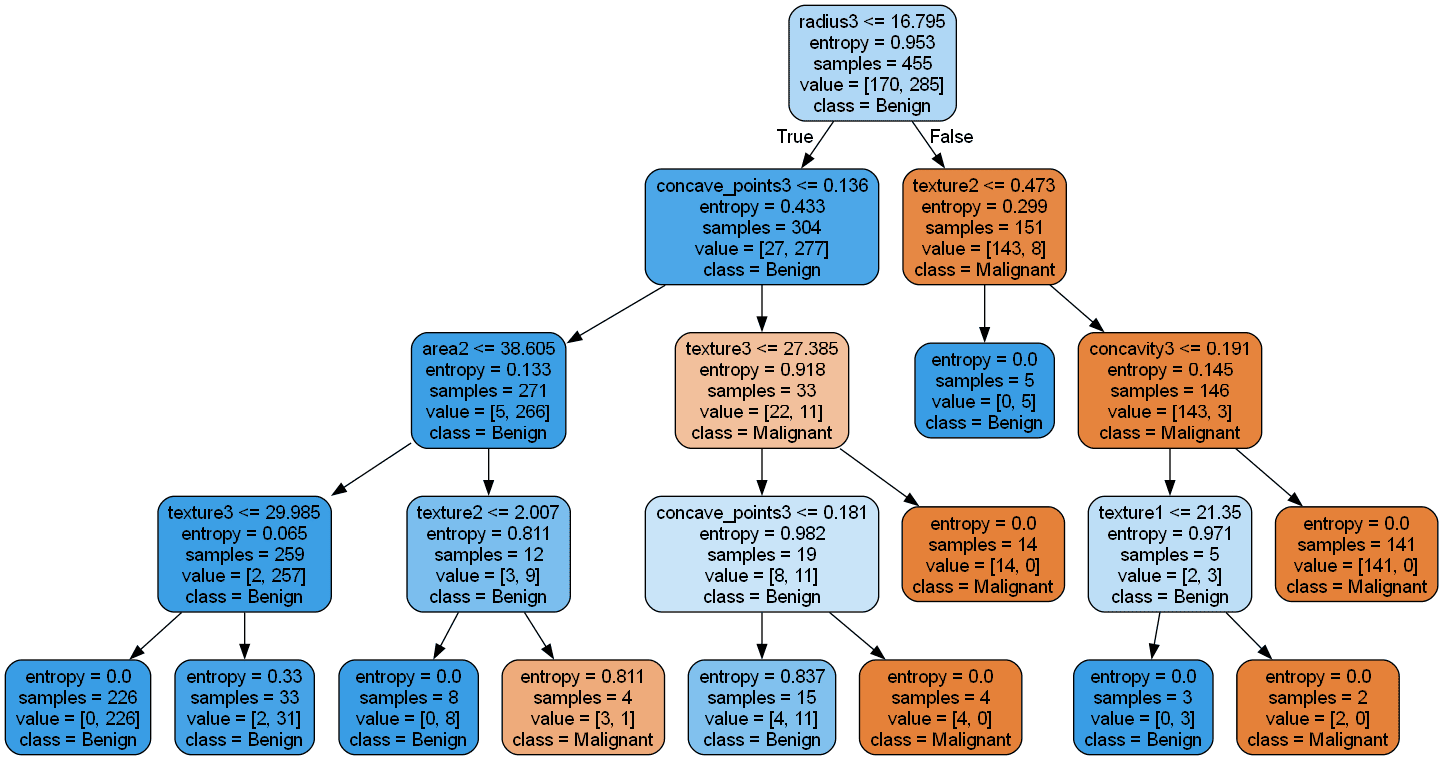
\includegraphics[width=0.65\textwidth]{imgs/dt-mini/dt__breast_cancer__80_vs_20__4.png}
	\caption{Breast Cancer: decision tree with \texttt{max\_depth}=4 (80/20 split).}\label{fig:bc-dt-depth-4}
\end{figure}

\begin{figure}[H]
	\centering
	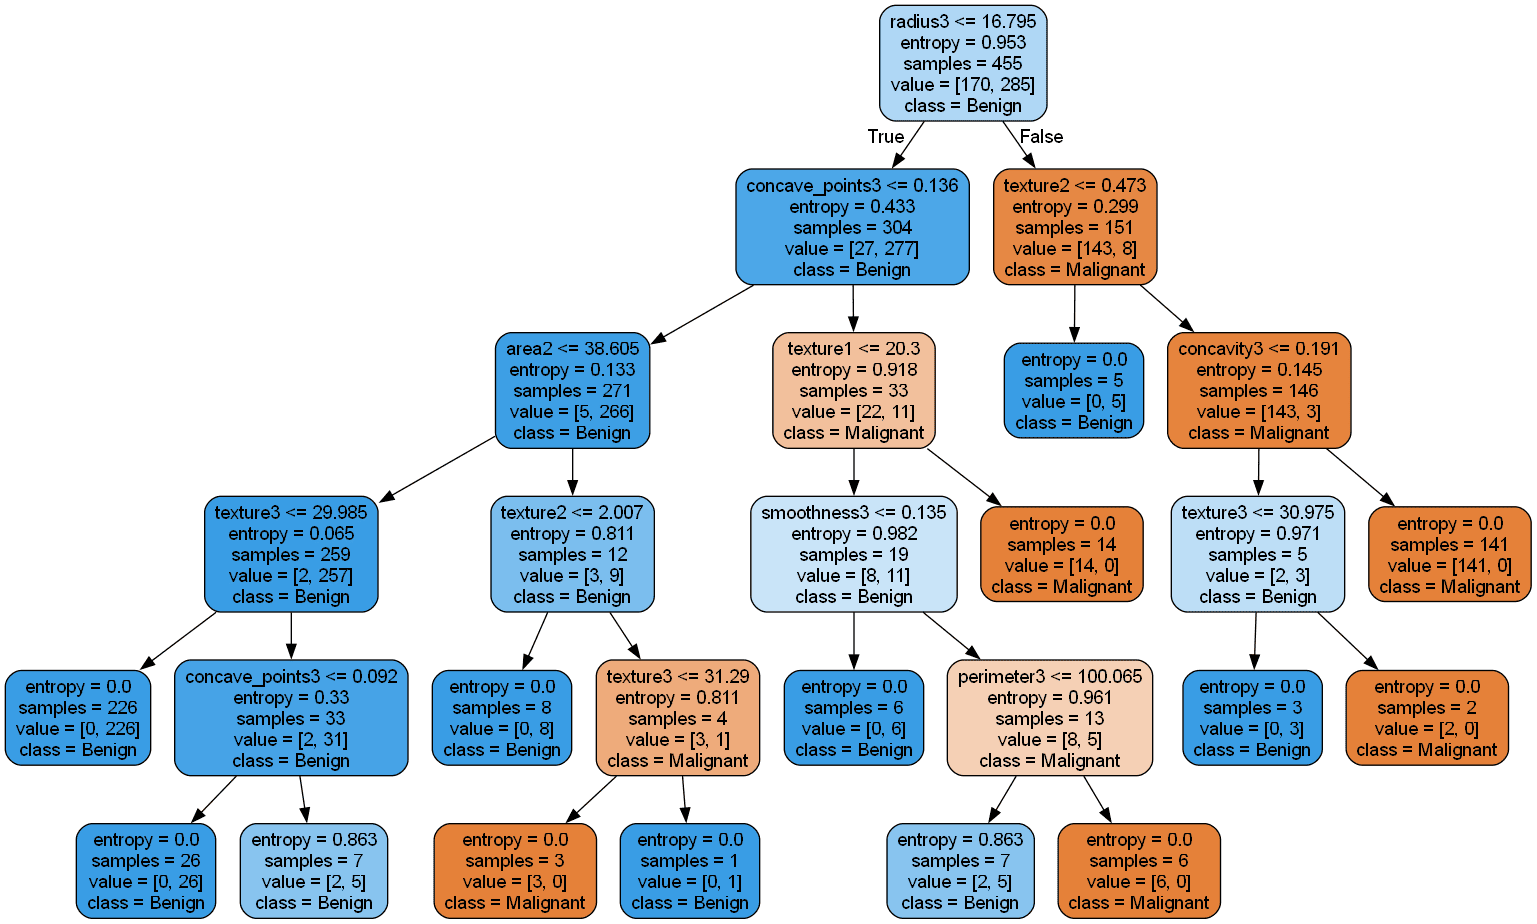
\includegraphics[width=0.65\textwidth]{imgs/dt-mini/dt__breast_cancer__80_vs_20__5.png}
	\caption{Breast Cancer: decision tree with \texttt{max\_depth}=5 (80/20 split).}\label{fig:bc-dt-depth-5}
\end{figure}

\begin{figure}[H]
	\centering
	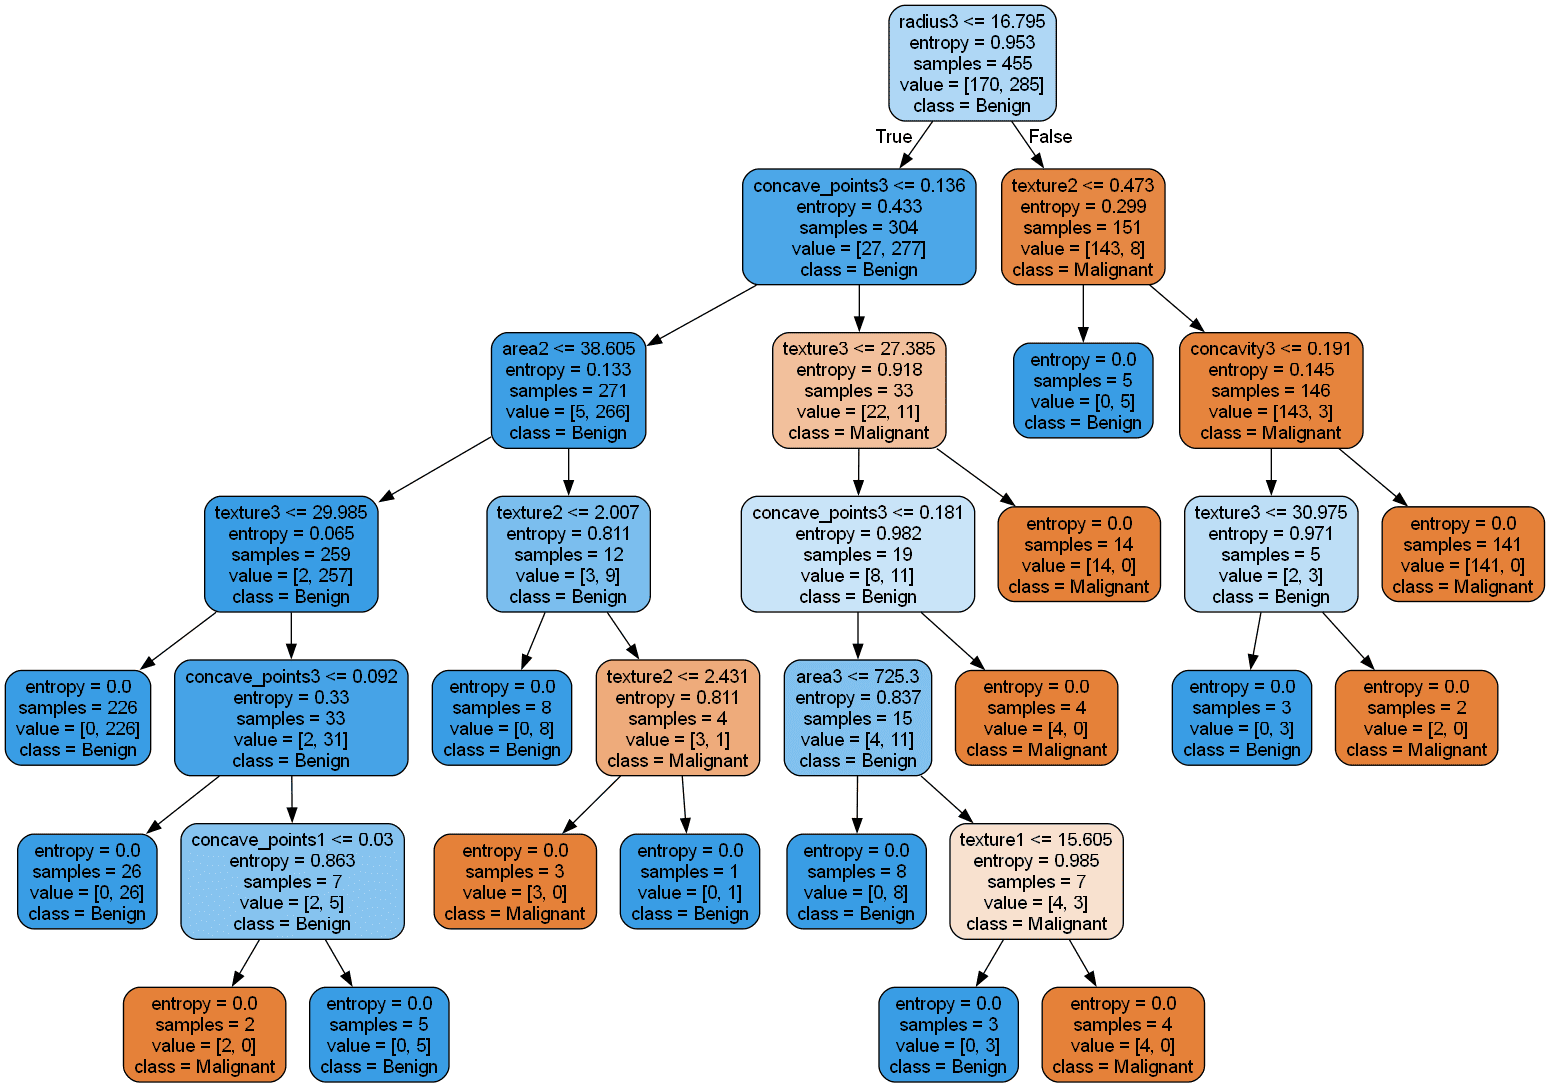
\includegraphics[width=0.65\textwidth]{imgs/dt-mini/dt__breast_cancer__80_vs_20__6.png}
	\caption{Breast Cancer: decision tree with \texttt{max\_depth}=6 (80/20 split).}\label{fig:bc-dt-depth-6}
\end{figure}

\begin{figure}[H]
	\centering
	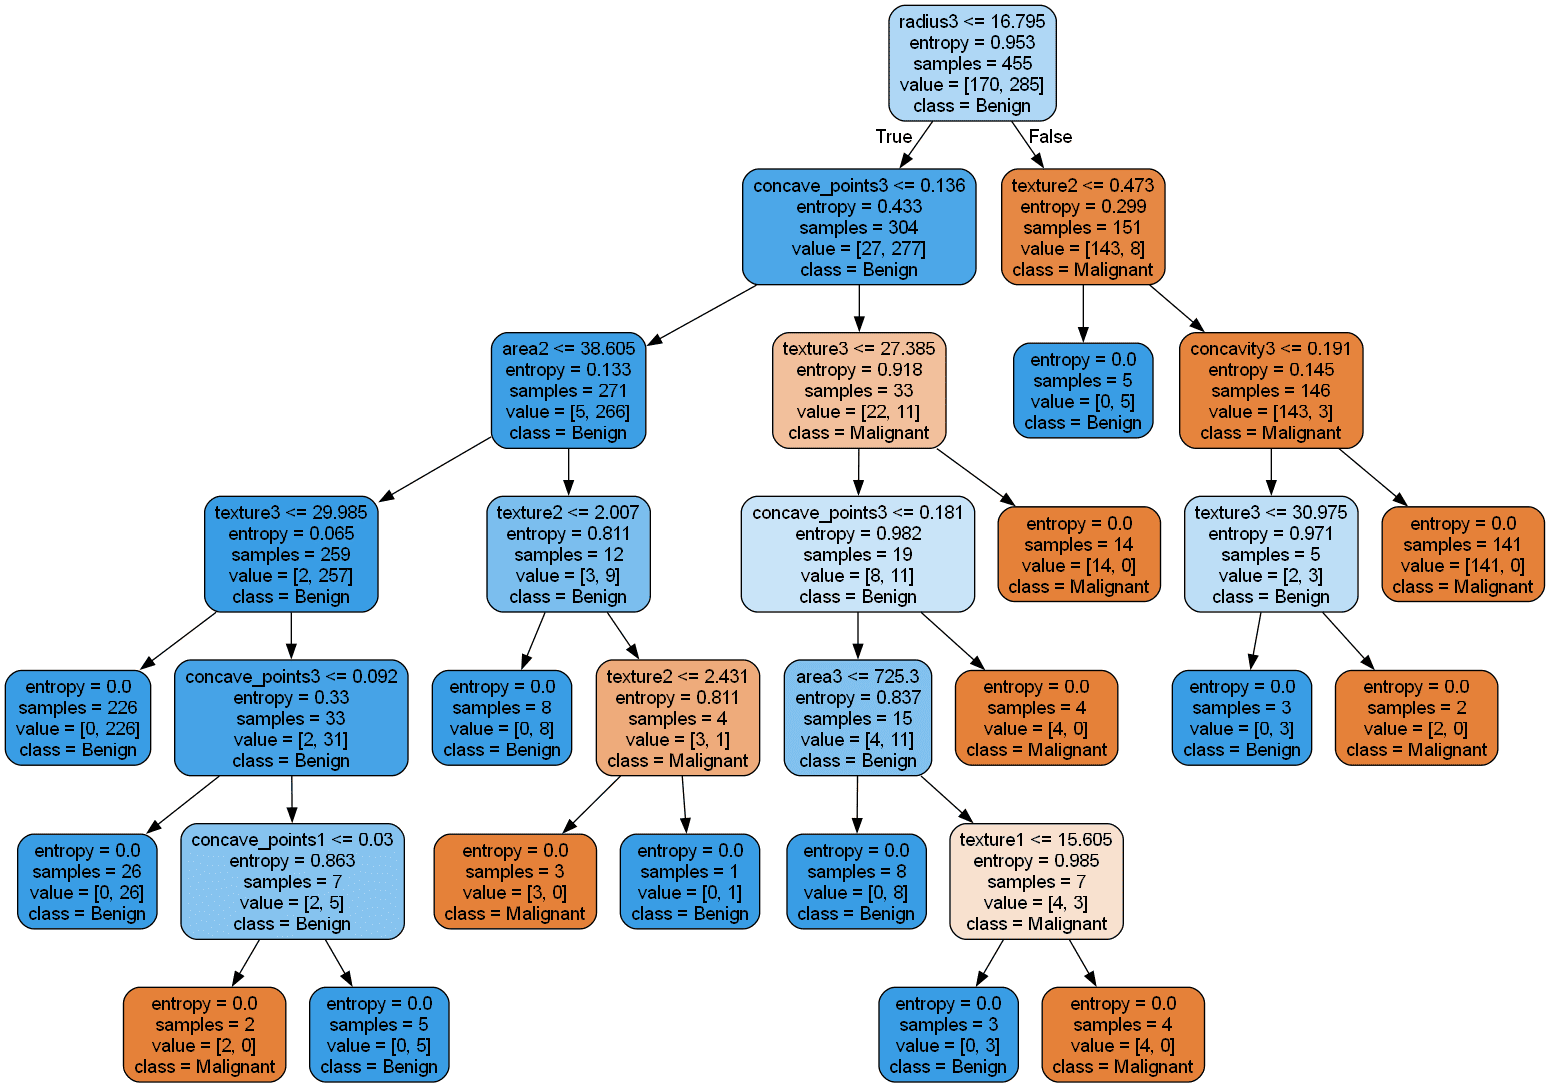
\includegraphics[width=0.65\textwidth]{imgs/dt-mini/dt__breast_cancer__80_vs_20__7.png}
	\caption{Breast Cancer: decision tree with \texttt{max\_depth}=7 (80/20 split).}\label{fig:bc-dt-depth-7}
\end{figure}

\begin{figure}[H]
	\centering
	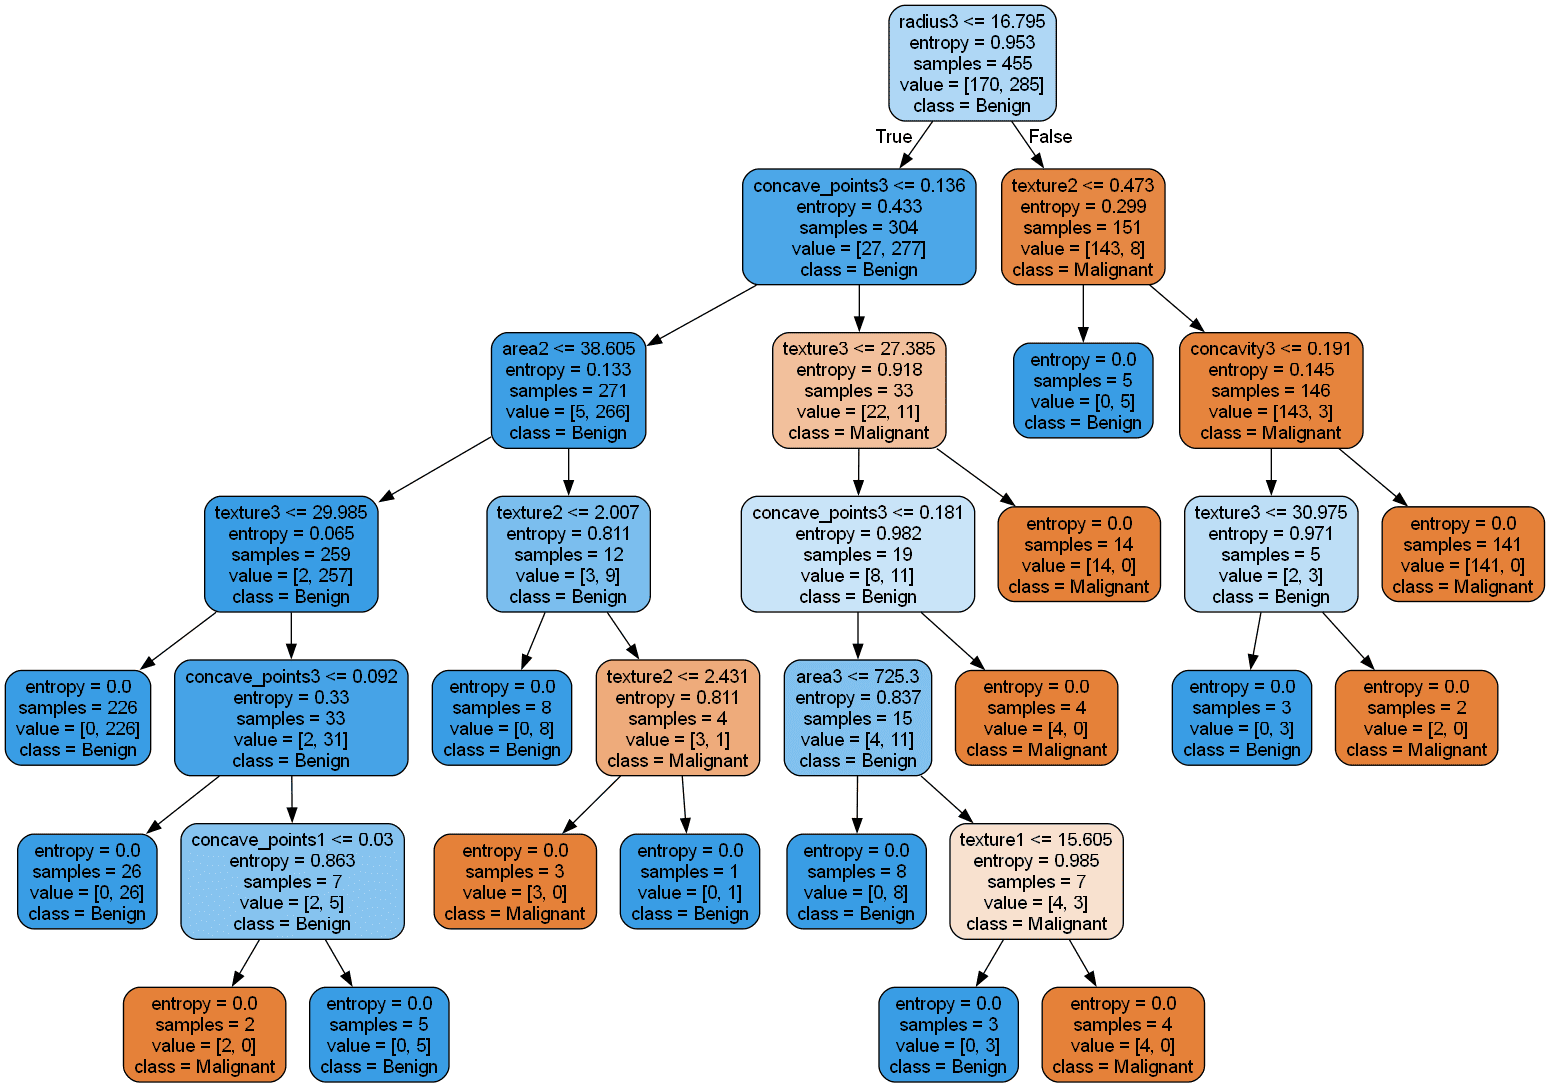
\includegraphics[width=0.65\textwidth]{imgs/dt-mini/dt__breast_cancer__80_vs_20__None.png}
	\caption{Breast Cancer: decision tree with \texttt{max\_depth}=None (80/20 split).}\label{fig:bc-dt-depth-none}
\end{figure}

\begin{figure}[H]
	\centering
	\begin{subfigure}{0.45\textwidth}
		\centering
		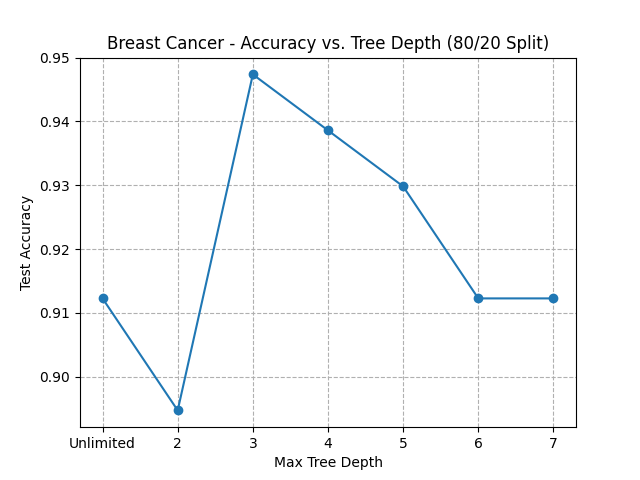
\includegraphics[width=\textwidth]{imgs/accuracy_vs_depth_breast_cancer.png}
	\end{subfigure}
	\hfill
	\begin{subfigure}{0.45\textwidth}
		\centering
		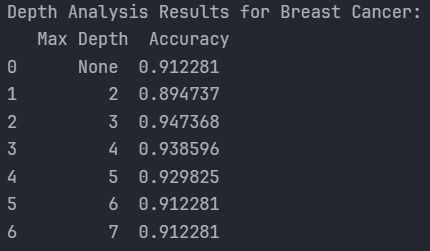
\includegraphics[width=\textwidth]{imgs/accuracy_vs_depth_breast_cancer__analysis.png}
	\end{subfigure}
\end{figure}

\subsubsection*{Insights - Depth and Accuracy}
\begin{itemize}
	\item \textbf{Underfitting at low depth:}
	      \texttt{max\_depth}=2 yields only \textbf{89.47\%} accuracy—too shallow to capture key interactions.
	\item \textbf{Optimal depth = 3:}
	      \begin{itemize}
		      \item Peaks at \textbf{94.74\%} ($\sim$5 pp gain over depth 2).
		      \item Balances bias/variance, capturing non-linear splits without overfitting.
	      \end{itemize}
	\item \textbf{Gradual overfitting beyond 3:}
	      \begin{itemize}
		      \item Depth 4: 93.86\%
		      \item Depth 5: 92.98\%
		      \item Depth 6, 7, None: all 91.23\%, matching the very deep tree but with far more complexity.
	      \end{itemize}
	\item \textbf{Interpretability trade-off:}
	      A 3-level tree has under 10 nodes—easy to explain—while delivering maximum generalization.
	\item \textbf{Recommendation:}
	      Limit \texttt{max\_depth} to \textbf{3-4} for this dataset to sustain high accuracy, control overfitting, and preserve model simplicity.
\end{itemize}

%================ Wine Quality =================%
\clearpage
\subsection{Wine Quality Dataset}
\subsubsection*{Dataset Description}
\begin{itemize}
	\item \textbf{Description:} The UCI Wine Quality dataset is used for classifying wine samples into quality levels based on physicochemical properties such as acidity, alcohol content, etc.
	\item \textbf{Dataset Info:} 4898 samples, with labels from 0 (low quality) to 10 (high quality).
	\item \textbf{Preprocessing:} shuffle \& stratified split at 40/60, 60/40, 80/20, 90/10.
\end{itemize}

\begin{figure}[H]
	\centering
	\begin{subfigure}{0.45\textwidth}
		\centering
		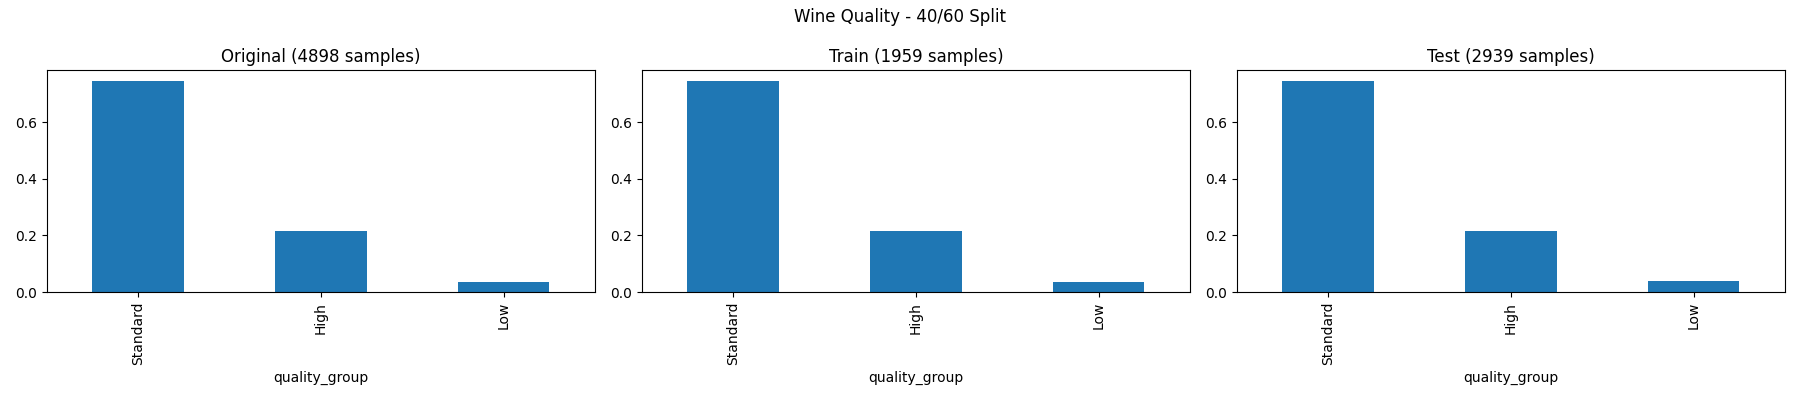
\includegraphics[width=\textwidth]{imgs/class_dist/class_dist__wine_quality__40_vs_60.png}
		\caption{Wine Quality: class distribution (40/60 split).}\label{fig:wq-cd-40-60}
	\end{subfigure}
	\hfill
	\begin{subfigure}{0.45\textwidth}
		\centering
		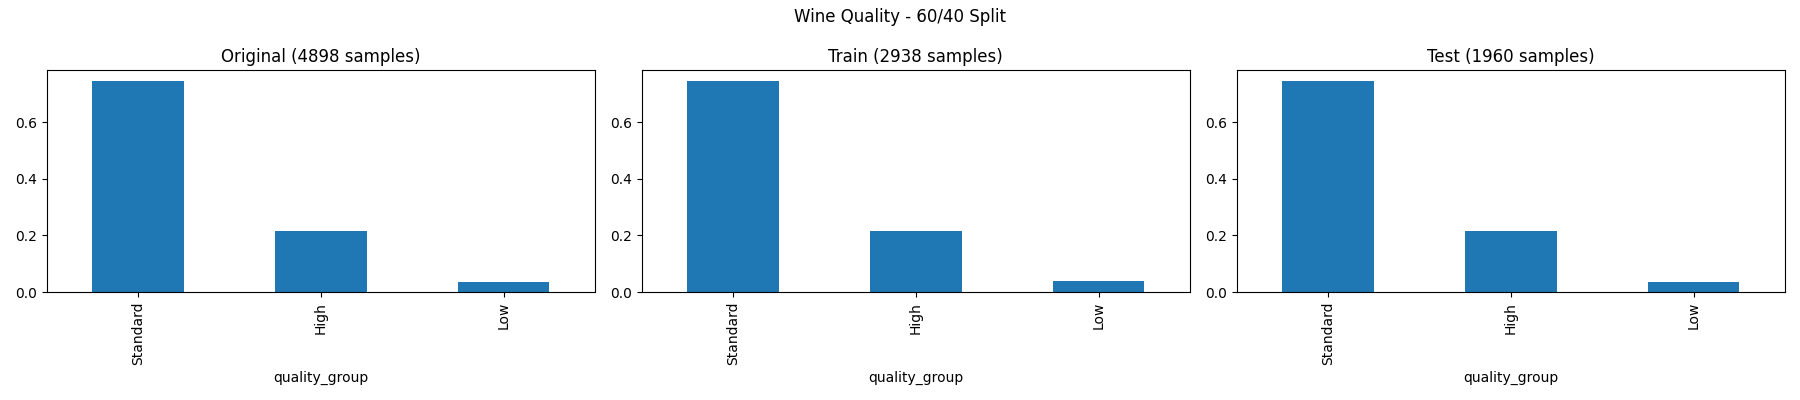
\includegraphics[width=\textwidth]{imgs/class_dist/class_dist__wine_quality__60_vs_40.png}
		\caption{Wine Quality: class distribution (60/40 split).}\label{fig:wq-cd-60-40}
	\end{subfigure}
	\hfill
	\begin{subfigure}{0.45\textwidth}
		\centering
		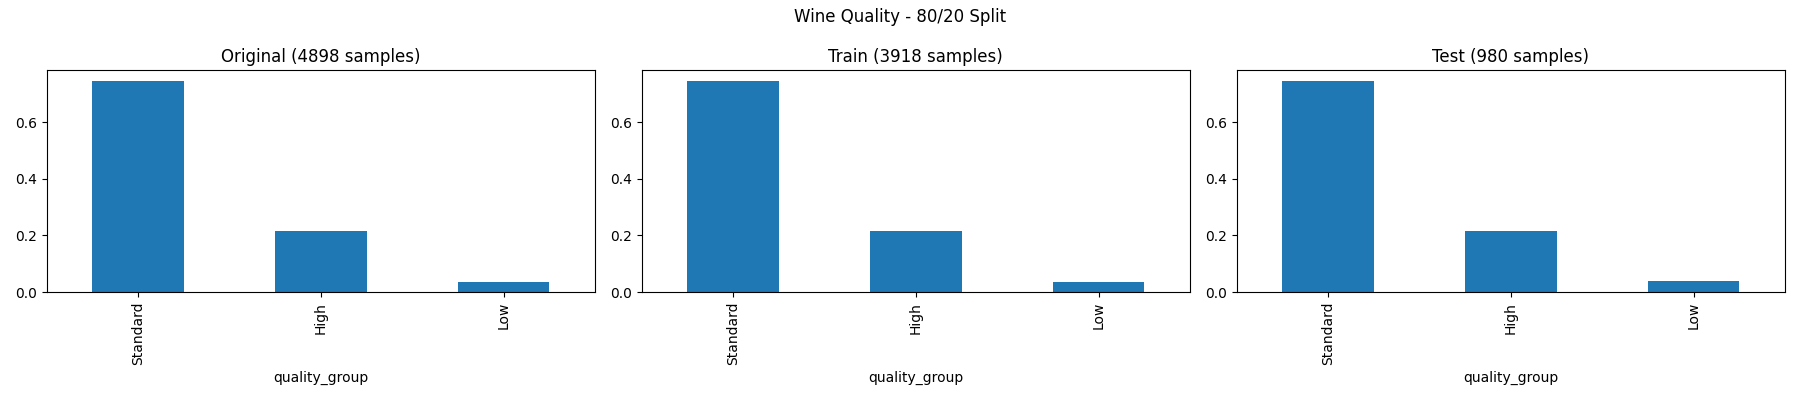
\includegraphics[width=\textwidth]{imgs/class_dist/class_dist__wine_quality__80_vs_20.png}
		\caption{Wine Quality: class distribution (80/20 split).}\label{fig:wq-cd-80-20}
	\end{subfigure}
	\hfill
	\begin{subfigure}{0.45\textwidth}
		\centering
		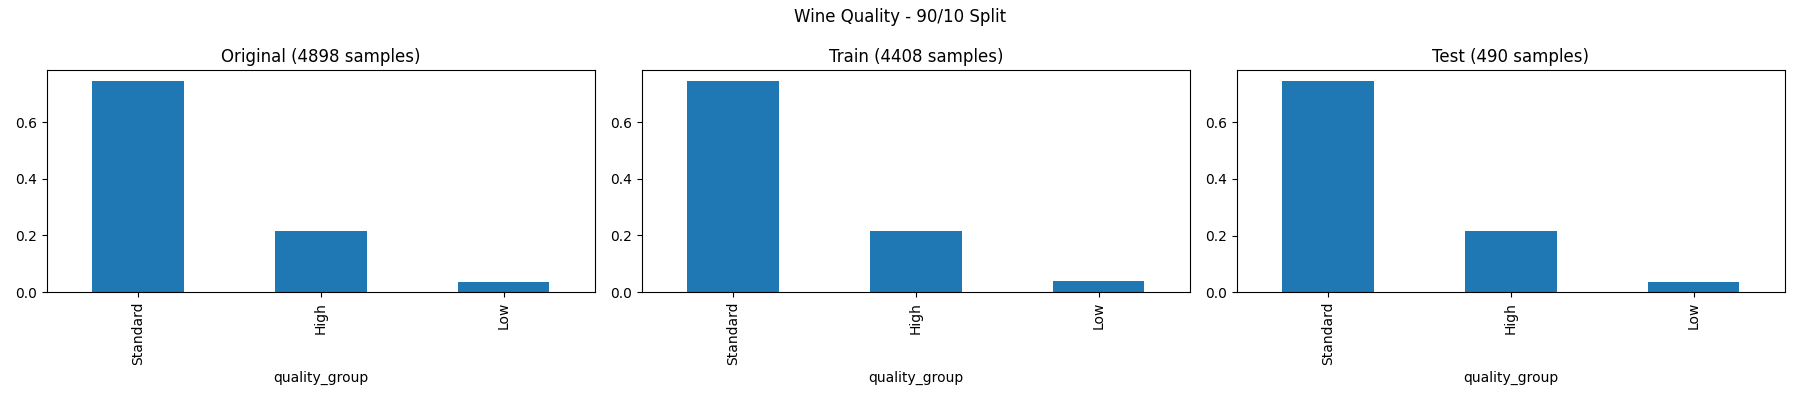
\includegraphics[width=\textwidth]{imgs/class_dist/class_dist__wine_quality__90_vs_10.png}
		\caption{Wine Quality: class distribution (90/10 split).}\label{fig:wq-cd-90-10}
	\end{subfigure}

	\caption{Class distributions}\label{fig:wq-cd-all}
\end{figure}

% \clearpage
% \subsubsection*{Building Decision Tree Classifiers for each train/test proportions}
% \begin{figure}[H]
% 	\centering
% 	\includegraphics[width=0.8\textwidth]{imgs/dt-mini/dt__wine_quality__40_vs_60.png}
% 	\caption{Wine Quality: decision tree for 40/60 split.}\label{fig:wq-dt-40-60}
% \end{figure}
% \begin{figure}[H]
% 	\centering
% 	\includegraphics[width=0.8\textwidth]{imgs/dt-mini/dt__wine_quality__60_vs_40.png}
% 	\caption{Wine Quality: decision tree for 60/40 split.}\label{fig:wq-dt-60-40}
% \end{figure}
% \begin{figure}[H]
% 	\centering
% 	\includegraphics[width=0.8\textwidth]{imgs/dt-mini/dt__wine_quality__80_vs_20.png}
% 	\caption{Wine Quality: decision tree for 80/20 split.}\label{fig:wq-dt-80-20}
% \end{figure}
% \begin{figure}[H]
% 	\centering
% 	\includegraphics[width=0.8\textwidth]{imgs/dt-mini/dt__wine_quality__90_vs_10.png}
% 	\caption{Wine Quality: decision tree for 90/10 split.}\label{fig:wq-dt-90-10}
% \end{figure}

\clearpage
\subsubsection*{Evaluating the decision tree classifiers}
\begin{figure}[H]
	\centering
	\begin{subfigure}{0.45\textwidth}
		\centering
		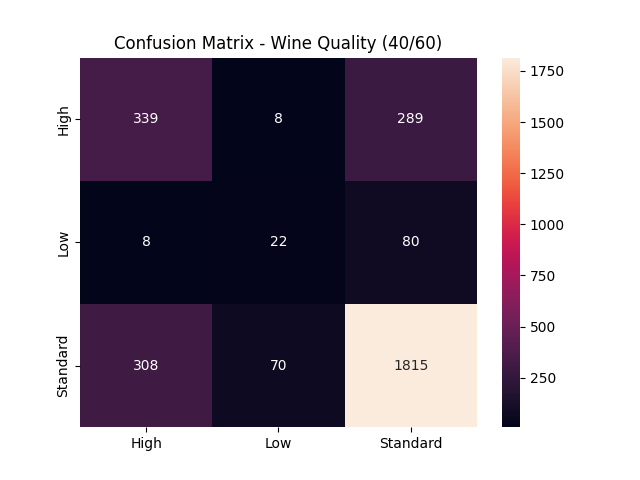
\includegraphics[width=\textwidth]{imgs/confusion_mat/confusion_mat__wine_quality__40_vs_60.png}
		\caption{Wine Quality: confusion matrix (40/60 split).}\label{fig:wq-cm-40-60}
	\end{subfigure}
	\hfill
	\begin{subfigure}{0.45\textwidth}
		\centering
		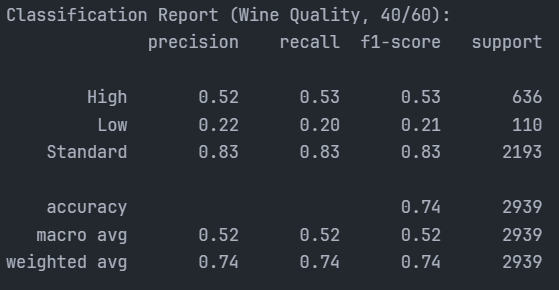
\includegraphics[width=\textwidth]{imgs/confusion_mat/class_rp__wine_quality__40_vs_60.png}
		\caption{Wine Quality: Classification Report (40/60 split).}\label{fig:wq-cr-40-60}
	\end{subfigure}

	\caption{Classification Report and Confusion Matrix (40/60 split)}\label{fig:wq-eval-40-60}
\end{figure}
\begin{figure}[H]
	\centering
	\begin{subfigure}{0.45\textwidth}
		\centering
		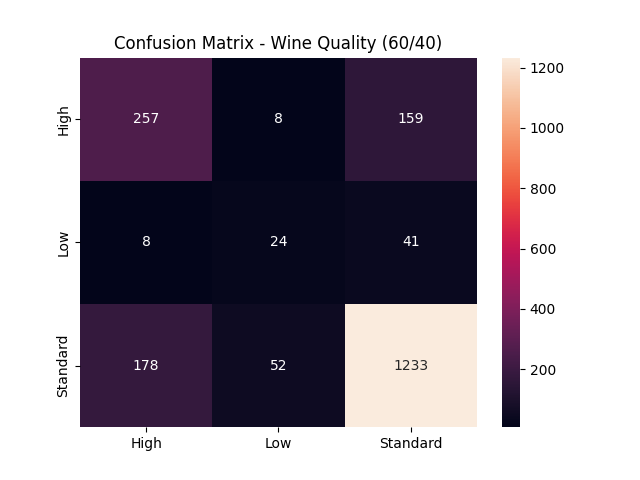
\includegraphics[width=\textwidth]{imgs/confusion_mat/confusion_mat__wine_quality__60_vs_40.png}
		\caption{Wine Quality: confusion matrix (60/40 split).}\label{fig:wq-cm-60-40}
	\end{subfigure}
	\hfill
	\begin{subfigure}{0.45\textwidth}
		\centering
		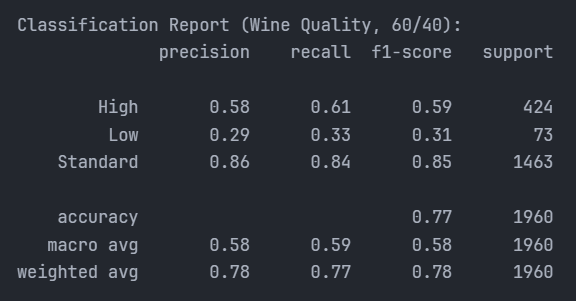
\includegraphics[width=\textwidth]{imgs/confusion_mat/class_rp__wine_quality__60_vs_40.png}
		\caption{Wine Quality: Classification Report (60/40 split).}\label{fig:wq-cr-60-40}
	\end{subfigure}

	\caption{Classification Report and Confusion Matrix (60/40 split)}\label{fig:wq-eval-60-40}
\end{figure}
\begin{figure}[H]
	\centering
	\begin{subfigure}{0.45\textwidth}
		\centering
		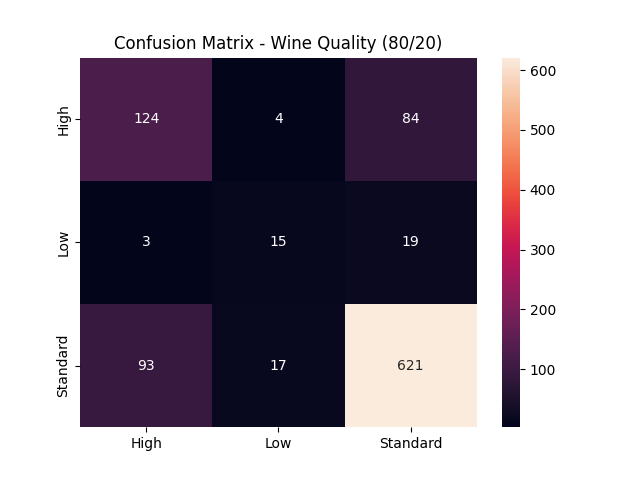
\includegraphics[width=\textwidth]{imgs/confusion_mat/confusion_mat__wine_quality__80_vs_20.png}
		\caption{Wine Quality: confusion matrix (80/20 split).}\label{fig:wq-cm-80-20}
	\end{subfigure}
	\hfill
	\begin{subfigure}{0.45\textwidth}
		\centering
		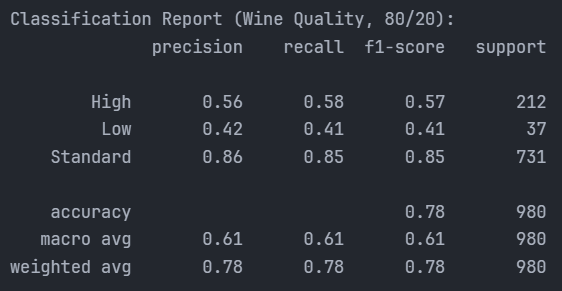
\includegraphics[width=\textwidth]{imgs/confusion_mat/class_rp__wine_quality__80_vs_20.png}
		\caption{Wine Quality: Classification Report (80/20 split).}\label{fig:wq-cr-80-20}
	\end{subfigure}

	\caption{Classification Report and Confusion Matrix (80/20 split)}\label{fig:wq-eval-80-20}
\end{figure}
\begin{figure}[H]
	\centering
	\begin{subfigure}{0.45\textwidth}
		\centering
		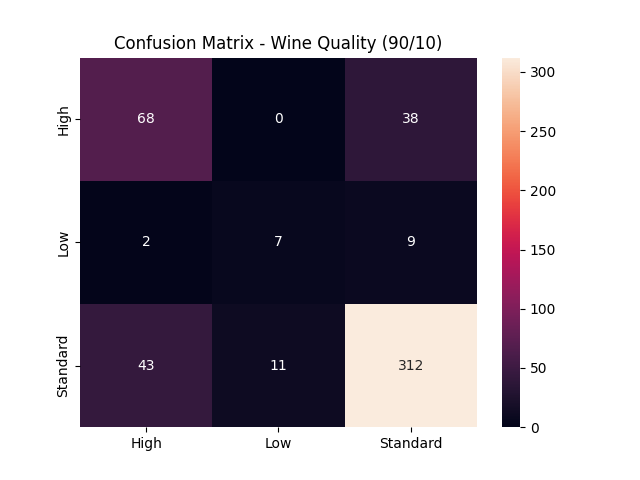
\includegraphics[width=\textwidth]{imgs/confusion_mat/confusion_mat__wine_quality__90_vs_10.png}
		\caption{Wine Quality: confusion matrix (90/10 split).}\label{fig:wq-cm-90-10}
	\end{subfigure}
	\hfill
	\begin{subfigure}{0.45\textwidth}
		\centering
		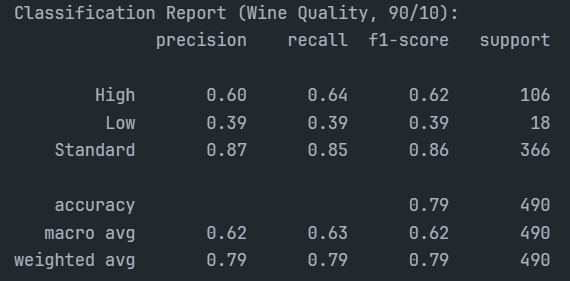
\includegraphics[width=\textwidth]{imgs/confusion_mat/class_rp__wine_quality__90_vs_10.png}
		\caption{Wine Quality: Classification Report (90/10 split).}\label{fig:wq-cr-90-10}
	\end{subfigure}

	\caption{Classification Report and Confusion Matrix (90/10 split)}\label{fig:wq-eval-90-10}
\end{figure}


\subsubsection*{Insights - Performance Evaluation}
\begin{itemize}
	\item \textbf{Overall accuracy trend:}
	      \begin{itemize}
		      \item Rises steadily from \textbf{74\%} (40/60) → \textbf{77\%} (60/40) → \textbf{78\%} (80/20) → \textbf{79\%} (90/10).
		      \item Larger training sets consistently improve generalization.
	      \end{itemize}
	\item \textbf{Class-level performance:}
	      \begin{itemize}
		      \item \emph{Standard (majority) class:}
		            \begin{itemize}
			            \item Precision/recall \(\approx0.83\) at 40/60, rising to \(approx0.87\) at 90/10.
			            \item High support (2,193→366) yields consistently strong F1-scores (0.83 → 0.86).
		            \end{itemize}
		      \item \emph{High quality:}
		            \begin{itemize}
			            \item Precision improves from 0.52 → 0.60; recall from 0.53 → 0.64 as training size grows.
			            \item Indicates better detection of top‐tier wines with more data.
		            \end{itemize}
		      \item \emph{Low quality:}
		            \begin{itemize}
			            \item Lowest metrics: precision 0.22 → 0.39, recall 0.20 → 0.39 across splits.
			            \item Small support (110→18) makes “Low” wines hardest to classify.
		            \end{itemize}
	      \end{itemize}
	\item \textbf{Macro vs.\ weighted averages:}
	      \begin{itemize}
		      \item Macro-avg F1 climbs from 0.52 → 0.62, reflecting improvement on minority classes.
		      \item Weighted-avg F1 follows overall accuracy closely (0.74 → 0.79).
	      \end{itemize}
	\item \textbf{Class imbalance impact:}
	      The dominant “Standard” category (\(\approx70\%\) of samples) drives overall accuracy; minority classes require targeted strategies (e.g.\ class weighting) for balanced performance.
\end{itemize}

\clearpage
\subsubsection*{Decision Tree Classifier with Different Depths}
\begin{figure}[H]
	\centering
	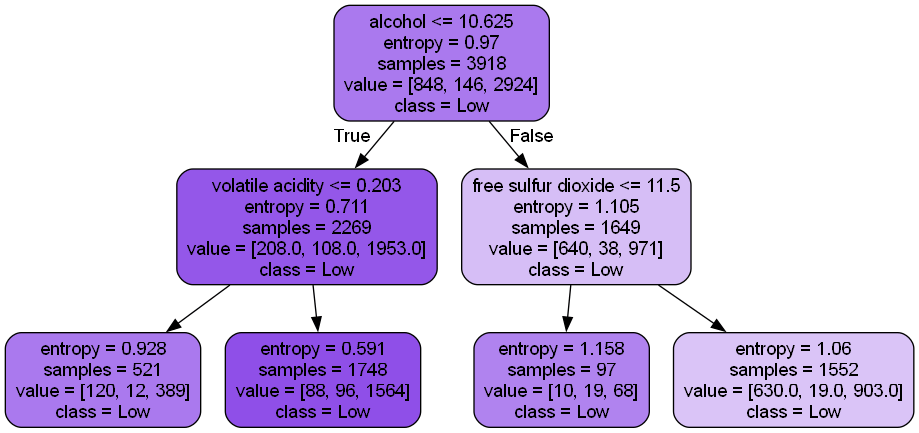
\includegraphics[width=0.65\textwidth]{imgs/dt-mini/dt__wine_quality__80_vs_20__2.png}
	\caption{Wine Quality: decision tree with \texttt{max\_depth}=2 (80/20 split).}\label{fig:wq-dt-depth-2}
\end{figure}

\begin{figure}[H]
	\centering
	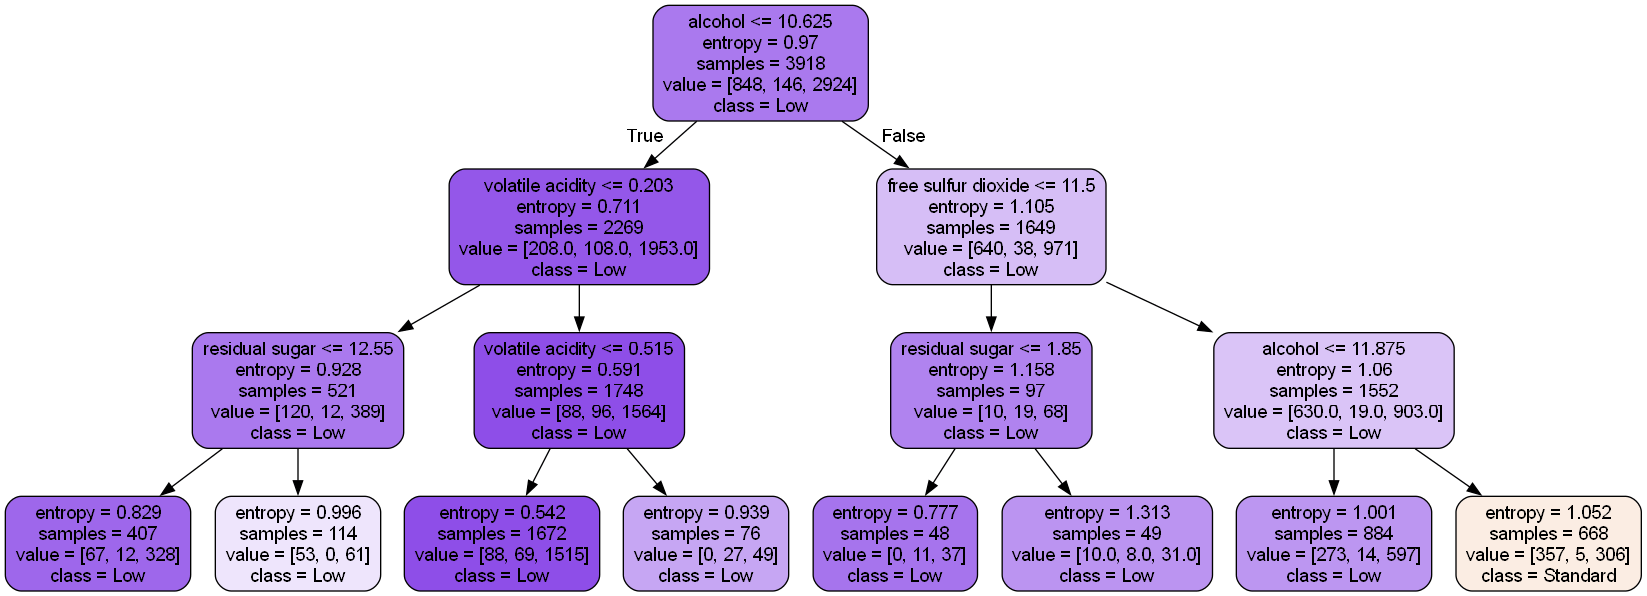
\includegraphics[width=0.65\textwidth]{imgs/dt-mini/dt__wine_quality__80_vs_20__3.png}
	\caption{Wine Quality: decision tree with \texttt{max\_depth}=3 (80/20 split).}\label{fig:wq-dt-depth-3}
\end{figure}

\begin{figure}[H]
	\centering
	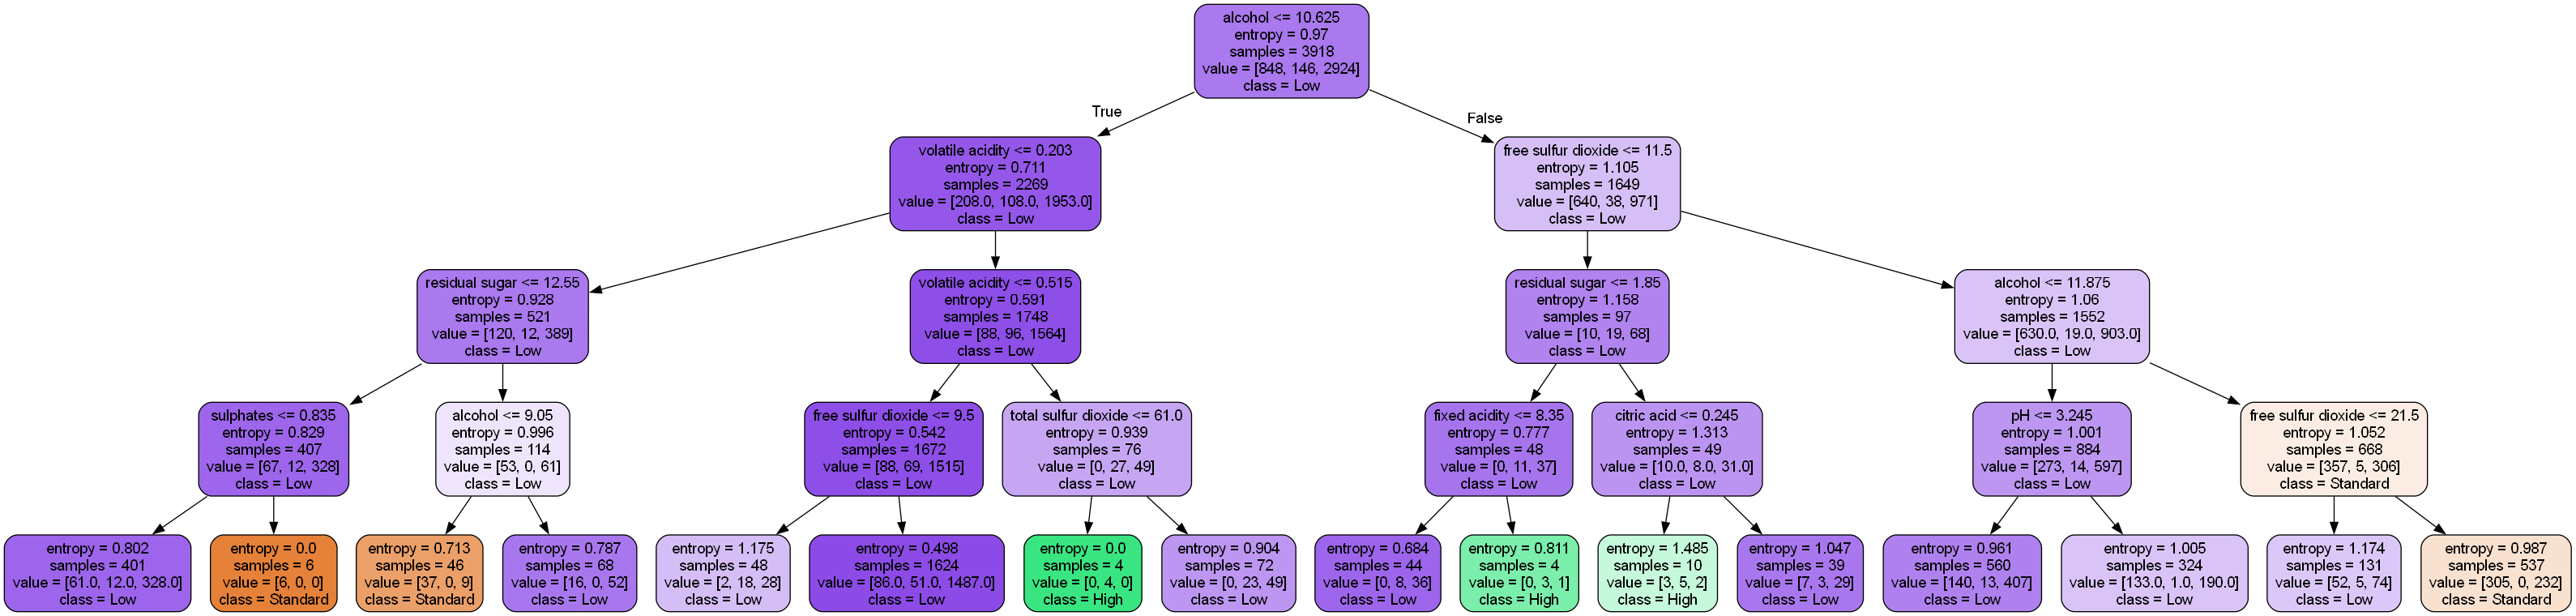
\includegraphics[width=0.65\textwidth]{imgs/dt-mini/dt__wine_quality__80_vs_20__4.png}
	\caption{Wine Quality: decision tree with \texttt{max\_depth}=4 (80/20 split).}\label{fig:wq-dt-depth-4}
\end{figure}

\begin{figure}[H]
	\centering
	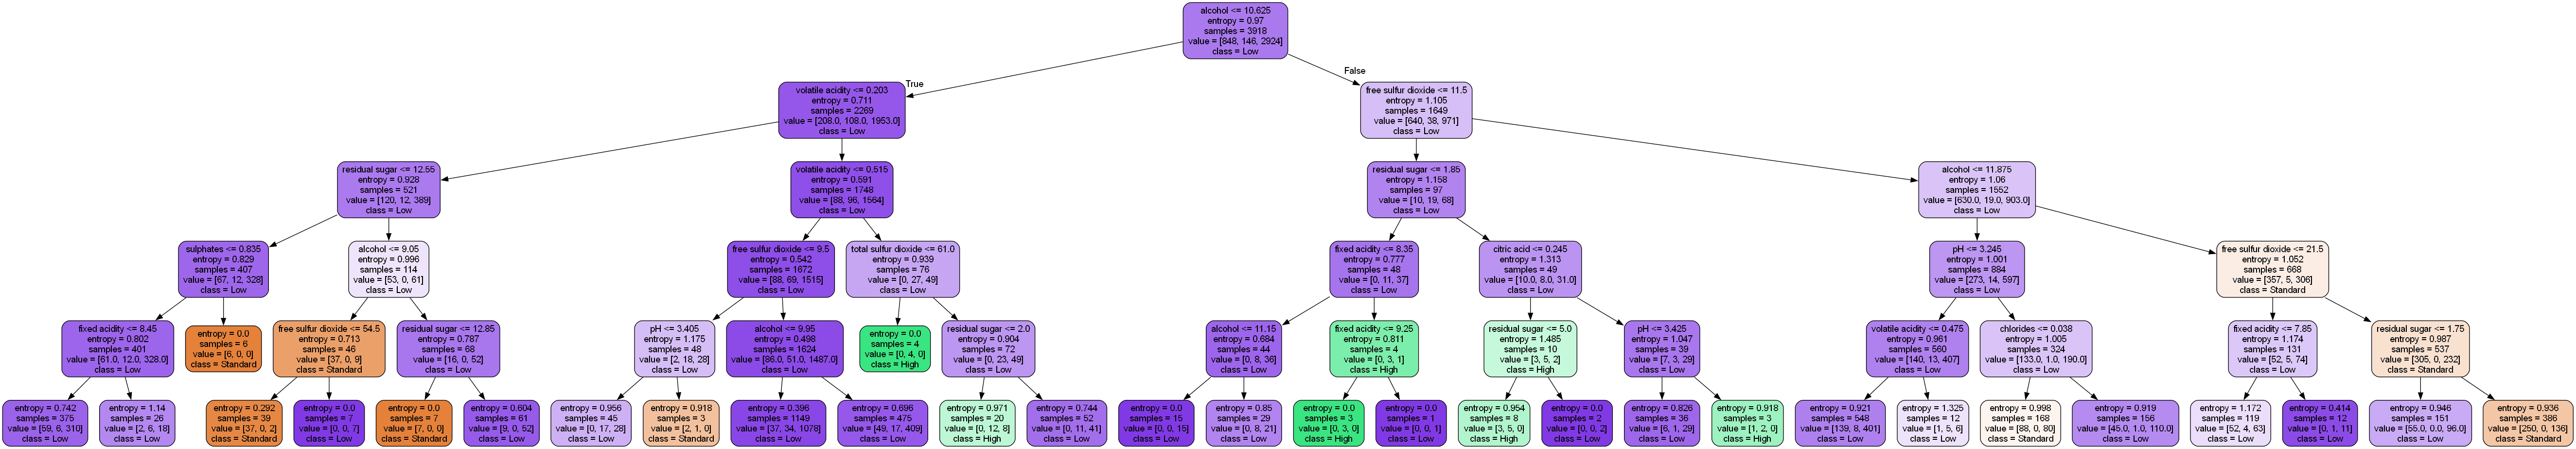
\includegraphics[width=0.65\textwidth]{imgs/dt-mini/dt__wine_quality__80_vs_20__5.png}
	\caption{Wine Quality: decision tree with \texttt{max\_depth}=5 (80/20 split).}\label{fig:wq-dt-depth-5}
\end{figure}

\begin{figure}[H]
	\centering
	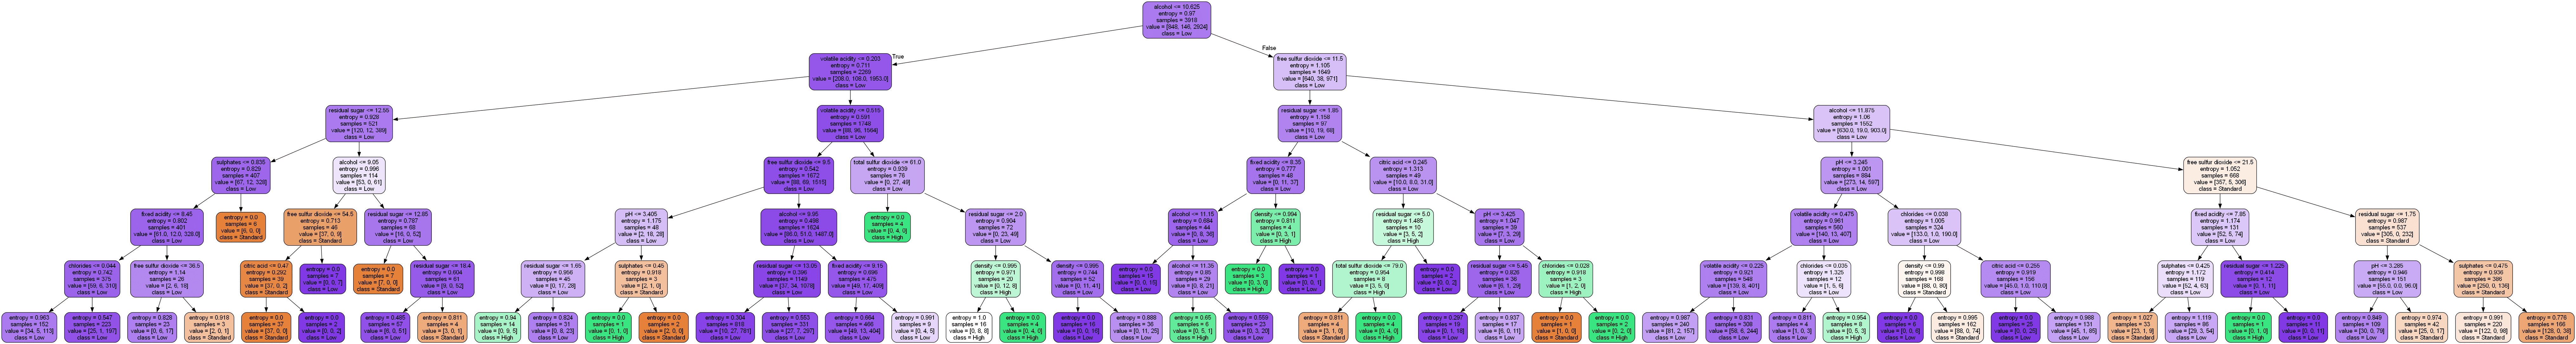
\includegraphics[width=0.65\textwidth]{imgs/dt-mini/dt__wine_quality__80_vs_20__6.png}
	\caption{Wine Quality: decision tree with \texttt{max\_depth}=6 (80/20 split).}\label{fig:wq-dt-depth-6}
\end{figure}

\begin{figure}[H]
	\centering
	
\includegraphics[width=0.65\textwidth]{imgs/dt-mini/dt__wine_quality__80_vs_20__7.png}
	\caption{Wine Quality: decision tree with \texttt{max\_depth}=7 (80/20 split).}\label{fig:wq-dt-depth-7}
\end{figure}

% \begin{figure}[H]
% 	\centering
% 	\includegraphics[width=0.8\textwidth]{imgs/dt-mini/dt__wine_quality__80_vs_20__None.png}
% 	\caption{Wine Quality: decision tree with \texttt{max\_depth}=None (80/20 split).}\label{fig:wq-dt-depth-none}
% \end{figure}

\begin{figure}[H]
	\centering
	\begin{subfigure}{0.45\textwidth}
		\centering
		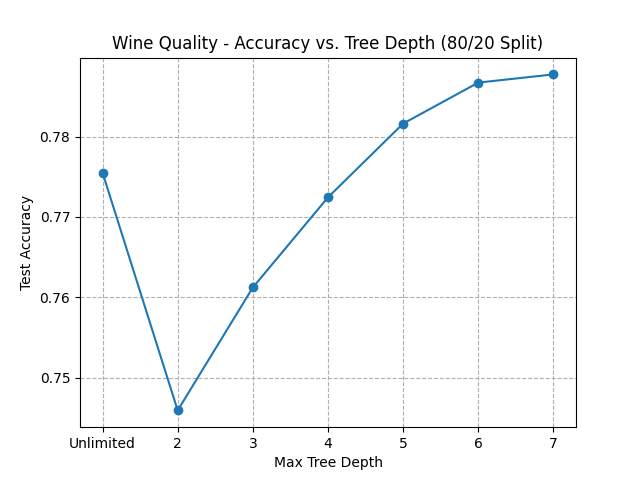
\includegraphics[width=\textwidth]{imgs/accuracy_vs_depth_wine_quality.png}
	\end{subfigure}
	\hfill
	\begin{subfigure}{0.45\textwidth}
		\centering
		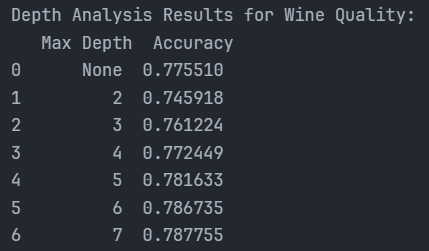
\includegraphics[width=\textwidth]{imgs/accuracy_vs_depth_wine_quality__analysis.png}
	\end{subfigure}
\end{figure}

\subsubsection*{Insights - Depth and Accuracy}
\begin{itemize}
	\item \textbf{Underfitting at low depth:}
	      \texttt{max\_depth}=2 yields only \textbf{74.6\%} accuracy, failing to capture interactions among acidity, alcohol, and sulphates.
	\item \textbf{Steady gains with depth:}
	      \begin{itemize}
		      \item Depth 3 → \textbf{76.0\%} (+1.5 pp),
		      \item Depth 4 → \textbf{77.0\%} (+1.1 pp),
		      \item Depth 5 → \textbf{78.2\%} (+0.9 pp).
		      \item Depth 6 → \textbf{78.7\%} (+0.6 pp),
		      \item Depth 7 → \textbf{78.8\%} (+0.1 pp).
	      \end{itemize}
	\item \textbf{Unrestricted tree underperforms:}
	      The fully grown tree (None) reaches \textbf{77.6\%}, below depth 7, indicating pruning aids generalization.
	\item \textbf{Optimal depth range:}
	      Depth 5-7 balances complexity and predictive power; marginal gains beyond depth 6 suggest diminishing returns.
	\item \textbf{Practical recommendation:}
	      For multi-class wine quality prediction, set \texttt{max\_depth} around \textbf{6} to maximize test accuracy while keeping the tree interpretable.
\end{itemize}


%================ Car Evaluation =================%
\clearpage
\subsection{Car Evaluation Dataset}
\subsubsection*{Dataset Description}
\begin{itemize}
	\item \textbf{Description:} Car Evaluation Database was derived from a simple hierarchical decision model originally developed for the demonstration of DEX, M. Bohanec, V. Rajkovic: Expert system for decision making.
	\item \textbf{Dataset Info:} 1728 samples, 4 classes (unacc, acc, good, vgood), 6 categorical attributes (buying price, maintenance cost, doors, etc.).
	\item \textbf{Preprocessing:} shuffle \& stratified split at 40/60, 60/40, 80/20, 90/10.
\end{itemize}

\begin{figure}[H]
	\centering
	\begin{subfigure}{0.45\textwidth}
		\centering
		\includegraphics[width=\textwidth]{imgs/class_dist/class_dist__car_evaluation__40_vs_60.png}
		\caption{Car Evaluation: class distribution (40/60 split).}\label{fig:ce-cd-40-60}
	\end{subfigure}
	\hfill
	\begin{subfigure}{0.45\textwidth}
		\centering
		\includegraphics[width=\textwidth]{imgs/class_dist/class_dist__car_evaluation__60_vs_40.png}
		\caption{Car Evaluation: class distribution (60/40 split).}\label{fig:ce-cd-60-40}
	\end{subfigure}
	\hfill
	\begin{subfigure}{0.45\textwidth}
		\centering
		\includegraphics[width=\textwidth]{imgs/class_dist/class_dist__car_evaluation__80_vs_20.png}
		\caption{Car Evaluation: class distribution (80/20 split).}\label{fig:ce-cd-80-20}
	\end{subfigure}
	\hfill
	\begin{subfigure}{0.45\textwidth}
		\centering
		\includegraphics[width=\textwidth]{imgs/class_dist/class_dist__car_evaluation__90_vs_10.png}
		\caption{Car Evaluation: class distribution (90/10 split).}\label{fig:ce-cd-90-10}
	\end{subfigure}

	\caption{Class distributions}\label{fig:ce-cd-all}
\end{figure}

% \clearpage
% \subsubsection*{Building Decision Tree Classifiers for each train/test proportions}
% \begin{figure}[H]
% 	\centering
% 	\includegraphics[width=0.65\textwidth]{imgs/dt-mini/dt__car_evaluation__40_vs_60.png}
% 	\caption{Car Evaluation: decision tree for 40/60 split.}\label{fig:ce-dt-40-60}
% \end{figure}
% \begin{figure}[H]
% 	\centering
% 	\includegraphics[width=0.65\textwidth]{imgs/dt-mini/dt__car_evaluation__60_vs_40.png}
% 	\caption{Car Evaluation: decision tree for 60/40 split.}\label{fig:ce-dt-60-40}
% \end{figure}
% \begin{figure}[H]
% 	\centering
% 	\includegraphics[width=0.65\textwidth]{imgs/dt-mini/dt__car_evaluation__80_vs_20.png}
% 	\caption{Car Evaluation: decision tree for 80/20 split.}\label{fig:ce-dt-80-20}
% \end{figure}
% \begin{figure}[H]
% 	\centering
% 	\includegraphics[width=0.65\textwidth]{imgs/dt-mini/dt__car_evaluation__90_vs_10.png}
% 	\caption{Car Evaluation: decision tree for 90/10 split.}\label{fig:ce-dt-90-10}
% \end{figure}

\clearpage
\subsubsection*{Evaluating the decision tree classifiers}
\begin{figure}[H]
	\centering
	\begin{subfigure}{0.45\textwidth}
		\centering
		\includegraphics[width=\textwidth]{imgs/confusion_mat/confusion_mat__car_evaluation__40_vs_60.png}
		\caption{Car Evaluation: confusion matrix (40/60 split).}\label{fig:ce-cm-40-60}
	\end{subfigure}
	\hfill
	\begin{subfigure}{0.45\textwidth}
		\centering
		\includegraphics[width=\textwidth]{imgs/confusion_mat/class_rp__car_evaluation__40_vs_60.png}
		\caption{Car Evaluation: Classification Report (40/60 split).}\label{fig:ce-cr-40-60}
	\end{subfigure}

	\caption{Classification Report and Confusion Matrix (40/60 split)}\label{fig:ce-eval-40-60}
\end{figure}
\begin{figure}[H]
	\centering
	\begin{subfigure}{0.45\textwidth}
		\centering
		\includegraphics[width=\textwidth]{imgs/confusion_mat/confusion_mat__car_evaluation__60_vs_40.png}
		\caption{Car Evaluation: confusion matrix (60/40 split).}\label{fig:ce-cm-60-40}
	\end{subfigure}
	\hfill
	\begin{subfigure}{0.45\textwidth}
		\centering
		\includegraphics[width=\textwidth]{imgs/confusion_mat/class_rp__car_evaluation__60_vs_40.png}
		\caption{Car Evaluation: Classification Report (60/40 split).}\label{fig:ce-cr-60-40}
	\end{subfigure}

	\caption{Classification Report and Confusion Matrix (60/40 split)}\label{fig:ce-eval-60-40}
\end{figure}
\begin{figure}[H]
	\centering
	\begin{subfigure}{0.45\textwidth}
		\centering
		\includegraphics[width=\textwidth]{imgs/confusion_mat/confusion_mat__car_evaluation__80_vs_20.png}
		\caption{Car Evaluation: confusion matrix (80/20 split).}\label{fig:ce-cm-80-20}
	\end{subfigure}
	\hfill
	\begin{subfigure}{0.45\textwidth}
		\centering
		\includegraphics[width=\textwidth]{imgs/confusion_mat/class_rp__car_evaluation__80_vs_20.png}
		\caption{Car Evaluation: Classification Report (80/20 split).}\label{fig:ce-cr-80-20}
	\end{subfigure}

	\caption{Classification Report and Confusion Matrix (80/20 split)}\label{fig:ce-eval-80-20}
\end{figure}
\begin{figure}[H]
	\centering
	\begin{subfigure}{0.45\textwidth}
		\centering
		\includegraphics[width=\textwidth]{imgs/confusion_mat/confusion_mat__car_evaluation__90_vs_10.png}
		\caption{Car Evaluation: confusion matrix (90/10 split).}\label{fig:ce-cm-90-10}
	\end{subfigure}
	\hfill
	\begin{subfigure}{0.45\textwidth}
		\centering
		\includegraphics[width=\textwidth]{imgs/confusion_mat/class_rp__car_evaluation__90_vs_10.png}
		\caption{Car Evaluation: Classification Report (90/10 split).}\label{fig:ce-cr-90-10}
	\end{subfigure}

	\caption{Classification Report and Confusion Matrix (90/10 split)}\label{fig:ce-eval-90-10}
\end{figure}

\subsubsection*{Insights - Performance Evaluation}
\begin{itemize}
	\item \textbf{Accuracy by split ratio:}
	      \begin{itemize}
		      \item 40/60 split: \textbf{94\%}
		      \item 60/40 split: \textbf{98\%}
		      \item 80/20 split: \textbf{99\%}
		      \item 90/10 split: \textbf{99\%}
	      \end{itemize}
	      Accuracy rises sharply as the training set grows, peaking at 99\% when \(\geq80\%\) of data is used for training.
	\item \textbf{Class-level performance:}
	      \begin{itemize}
		      \item \emph{unacc (majority):} Precision and recall \(\geq98\%\) across all splits, reflecting the model's ease in identifying unacceptable cars.
		      \item \emph{acc:} Precision climbs from 88\% → 99\%, recall from 91\% → 100\% as training size increases, showing strong learning of the “acceptable” class.
		      \item \emph{good:}
		            \begin{itemize}
			            \item 40/60 split: Precision 71\%, Recall 59\% (support 41)
			            \item 60/40 split: Precision 96\%, Recall 89\% (support 28)
			            \item 80/20 split: Precision 88\%, Recall 100\% (support 14)
		            \end{itemize}
		            Smaller support for “good” leads to greater variance in its metrics.

		      \item \emph{vgood (minority):}
		            \begin{itemize}
			            \item Precision: 85-100\%
			            \item Recall by split:
			                  \begin{itemize}
				                  \item 40/60: 74\%
				                  \item 60/40: 96\%
				                  \item 80/20: 92\%
				                  \item 90/10: 86\%
			                  \end{itemize}
		            \end{itemize}
		            The recall swings reflect the model's difficulty detecting very‐good cars when examples are scarce.

	      \end{itemize}
	\item \textbf{Macro vs.\ weighted F1:}
	      \begin{itemize}
		      \item Macro-avg F1 improves from 83\% (40/60) → 96\% (60/40) → 97\% (80/20) → 96\% (90/10).
		      \item Weighted-avg F1 mirrors accuracy (94-99\%), driven by the dominant “unacc” class.
	      \end{itemize}
	\item \textbf{Class imbalance impact:} The “unacc” class (\(\approx70\%\) of samples) drives most of the overall accuracy. Minority classes (“good”, “vgood”) benefit greatly from more training data.
\end{itemize}

\clearpage
\subsubsection*{Decision Tree Classifier with Different Depths}
\begin{figure}[H]
	\centering
	\includegraphics[width=0.65\textwidth]{imgs/dt-mini/dt__car_evaluation__80_vs_20__2.png}
	\caption{Car Evaluation: decision tree with \texttt{max\_depth}=2 (80/20 split).}\label{fig:ce-dt-depth-2}
\end{figure}

\begin{figure}[H]
	\centering
	\includegraphics[width=0.65\textwidth]{imgs/dt-mini/dt__car_evaluation__80_vs_20__3.png}
	\caption{Car Evaluation: decision tree with \texttt{max\_depth}=3 (80/20 split).}\label{fig:ce-dt-depth-3}
\end{figure}

\begin{figure}[H]
	\centering
	\includegraphics[width=0.65\textwidth]{imgs/dt-mini/dt__car_evaluation__80_vs_20__4.png}
	\caption{Car Evaluation: decision tree with \texttt{max\_depth}=4 (80/20 split).}\label{fig:ce-dt-depth-4}
\end{figure}

\begin{figure}[H]
	\centering
	\includegraphics[width=0.65\textwidth]{imgs/dt-mini/dt__car_evaluation__80_vs_20__5.png}
	\caption{Car Evaluation: decision tree with \texttt{max\_depth}=5 (80/20 split).}\label{fig:ce-dt-depth-5}
\end{figure}

\begin{figure}[H]
	\centering
	\includegraphics[width=0.65\textwidth]{imgs/dt-mini/dt__car_evaluation__80_vs_20__6.png}
	\caption{Car Evaluation: decision tree with \texttt{max\_depth}=6 (80/20 split).}\label{fig:ce-dt-depth-6}
\end{figure}

\begin{figure}[H]
	\centering
	\includegraphics[width=0.65\textwidth]{imgs/dt-mini/dt__car_evaluation__80_vs_20__7.png}
	\caption{Car Evaluation: decision tree with \texttt{max\_depth}=7 (80/20 split).}\label{fig:ce-dt-depth-7}
\end{figure}

\begin{figure}[H]
	\centering
	\includegraphics[width=0.65\textwidth]{imgs/dt-mini/dt__car_evaluation__80_vs_20__None.png}
	\caption{Car Evaluation: decision tree with \texttt{max\_depth}=None (80/20 split).}\label{fig:ce-dt-depth-none}
\end{figure}

\begin{figure}[H]
	\centering
	\begin{subfigure}{0.45\textwidth}
		\centering
		\includegraphics[width=\textwidth]{imgs/accuracy_vs_depth_car_evaluation.png}
	\end{subfigure}
	\hfill
	\begin{subfigure}{0.45\textwidth}
		\centering
		\includegraphics[width=\textwidth]{imgs/accuracy_vs_depth_car_evaluation__analysis.png}
	\end{subfigure}
\end{figure}

\subsubsection*{Insights - Depth and Accuracy}
\begin{itemize}
	\item \textbf{Underfitting at shallow depths:}
	      \begin{itemize}
		      \item \texttt{max\_depth}=2: \textbf{78.0\%}
		      \item \texttt{max\_depth}=3: \textbf{80.6\%}
		      \item \texttt{max\_depth}=4: \textbf{79.8\%}
	      \end{itemize}
	      Very low depths cannot capture the multi-attribute categorical splits.
	\item \textbf{Rapid gains with moderate depth:}
	      \begin{itemize}
		      \item Depth 5: \textbf{87.0\%} (+8.2 pp over depth 4)
		      \item Depth 6: \textbf{86.7\%}
		      \item Depth 7: \textbf{93.4\%} (+6.7 pp over depth 6)
	      \end{itemize}
	      Indicates that deeper trees are needed to model complex combinations of the six categorical features.
	\item \textbf{Unrestricted tree (None):} \textbf{99.1\%}—the highest accuracy, achieving nearly perfect classification by fully expanding on all splits.
	\item \textbf{Interpretability vs.\ performance:}
	      \begin{itemize}
		      \item Limiting to depth 7 yields 93.4\% accuracy with a still-manageable tree size.
		      \item Allowing no limit pushes accuracy to 99.1\% at the cost of a very large, less interpretable tree.
	      \end{itemize}
	\item \textbf{Recommendation:}
	      \begin{itemize}
		      \item If maximum accuracy is required, use unrestricted depth.
		      \item For a balance of interpretability and high performance, cap \texttt{max\_depth} at \textbf{7}.
	      \end{itemize}
\end{itemize}
